\documentclass{beamer}
\usepackage[english]{babel}
\usepackage{graphicx}
\usepackage{multimedia}
\usepackage{hyperref}
\usepackage{subfigure}

\newcommand{\putat}[3]{\begin{picture}(0,0)(0,0)\put(#1,#2){#3}\end{picture}}
% Choose how your presentation looks.
%
% For more themes, color themes and font themes, see:
% http://deic.uab.es/~iblanes/beamer_gallery/index_by_theme.html
%
\mode<presentation>
{
  \usetheme{default}      % or try Darmstadt, Madrid, Warsaw, ...
  \usecolortheme{default} % or try albatross, beaver, crane, ...
  \usefonttheme{default}  % or try serif, structurebold, ...
  \setbeamertemplate{navigation symbols}{}
  \setbeamertemplate{caption}[numbered]
} 

\usepackage[english]{babel}
\usepackage[utf8x]{inputenc}

\title[Simultaneous Evolution of Morphology and Locomotion of Soft Robots by Novelty Search]{Simultaneous Evolution of Morphology and Locomotion of Soft Robots by Novelty Search}
\author{Georgios Methenitis}
\institute{UvA, ACT}
\date{\today}

\begin{document}

\begin{frame}
  \titlepage
\end{frame}

%\begin{frame}{Outline}
%  \tableofcontents
%\end{frame}



\section{Introduction}




\begin{frame}{Introduction}
\begin{block}{Soft Robots}
\begin{itemize}
\item Inspired by nature
\item Completely soft bodies
\item Capable of developing new kinds of locomotion
\end{itemize}
\end{block}
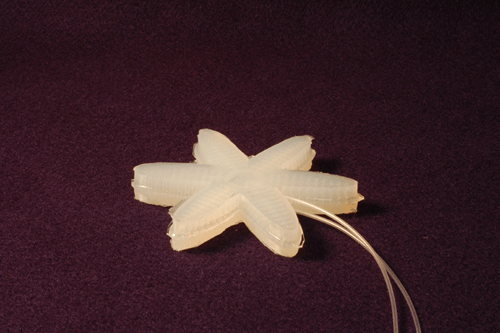
\includegraphics[width=0.3\textwidth,height=0.25\textheight]{../Figures/Misc/soft_robotics_figure.png}\		
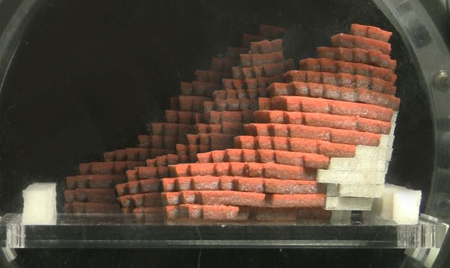
\includegraphics[width=0.3\textwidth,height=0.25\textheight]{../Figures/Misc/hillerPressureChamber.png}\	
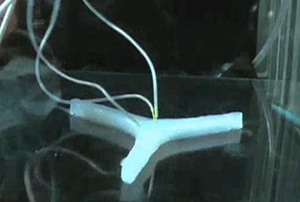
\includegraphics[width=0.3\textwidth,height=0.25\textheight]{../Figures/Misc/ExplodingRobot.jpg}\\
\vspace{0.3cm}
Soft robots can be actuated through air pressure tubes, environmental changes ( temperature, pressure ), even explosions.
\end{frame}






\section{Related Work}


\begin{frame}{Related Material}
\vspace{-1.5cm}
\begin{block}{
\includegraphics[scale=0.35]{../Figures/Misc/voxcad_logo.png}\	VoxCad Simulator~\cite{hiller2012dynamic}}
\begin{itemize}
\item Created by Jonathan Hiller and Hod Lipson
\item Voxel modeling and analyzing software
\end{itemize}
\end{block}
\putat{75}{-120}{\includegraphics[scale=0.12]{../Figures/Misc//voxcad.png}}
\begin{itemize}
\item Lattice
\item Voxels
\item Structure
\item Materials
\end{itemize}
\end{frame}

\begin{frame}[allowframebreaks]{Related Work}
\textit{Evolving virtual creature}s~\cite{sims1994evolving}
\begin{itemize}
\item Rigid body parts, joints
\item Evolution of the morphology and the control
\end{itemize}
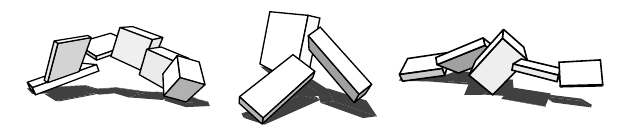
\includegraphics[scale=0.5]{../Figures/Misc/evolvingVirtualCreatures.png}\\
\textit{Evolving a diversity of virtual creatures through novelty search and local competition} ~\cite{lehman2011evolving}
\begin{itemize}
\item Same experimental framework
\item Novelty $<$ Fitness
\item Novelty search with global competition has the best average fitness.
\end{itemize}
\newpage
\textit{Evolving soft robots with multiple materials and a powerful generative encoding.}~\cite{cheney2013unshackling}
\begin{itemize}
\item Generative encoding, Compositional pattern-producing network, CPPN.
\item Neuroevolution of augmenting topologies, NEAT.
\end{itemize}
\vspace{0.3cm}
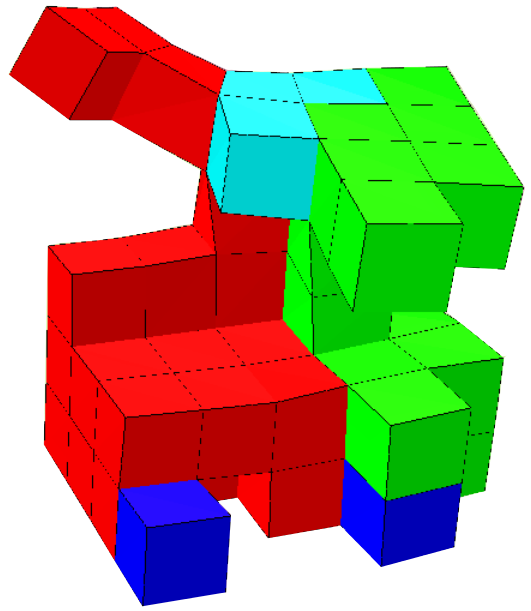
\includegraphics[width=0.3\textwidth,height=0.25\textheight]{../Figures/Misc/unshacklingEvolutionFigure1.png}\	\	\	
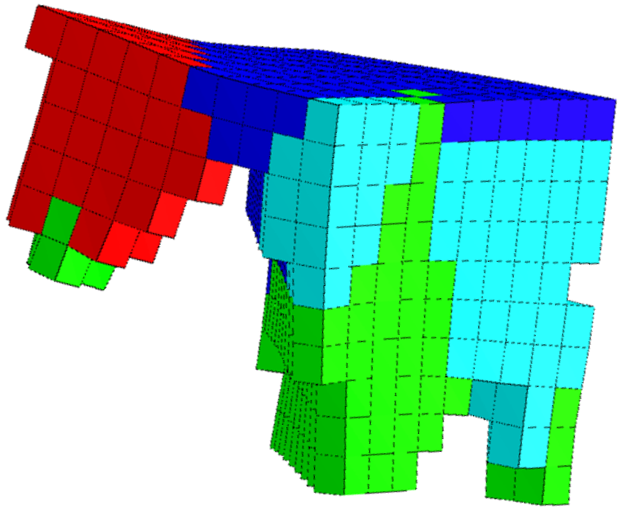
\includegraphics[width=0.3\textwidth,height=0.25\textheight]{../Figures/Misc/unshacklingEvolutionFigure2.png}\	\	\	
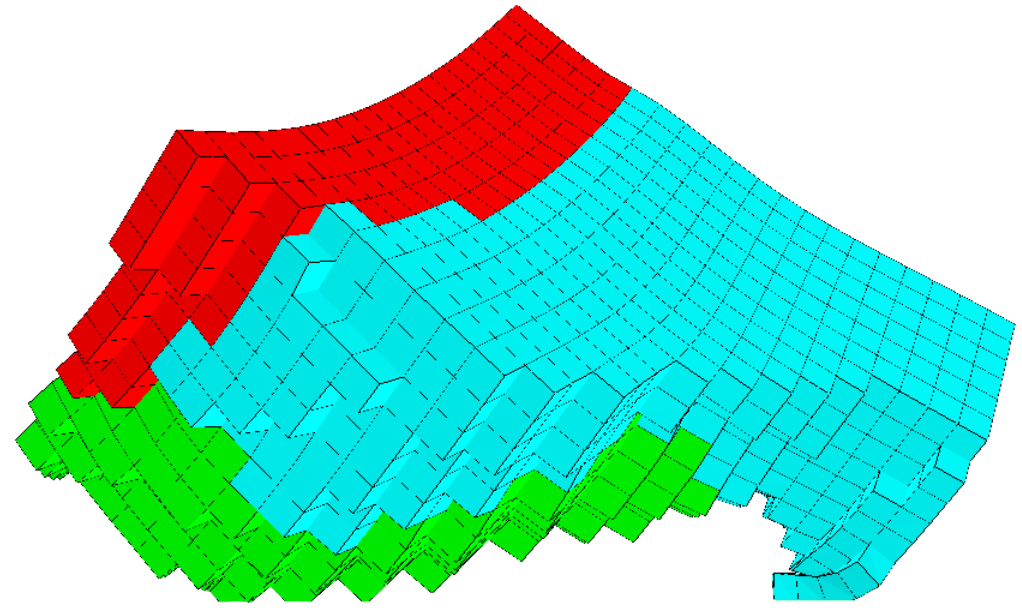
\includegraphics[width=0.3\textwidth,height=0.25\textheight]{../Figures/Misc/unshacklingEvolutionFigure3.png}
\end{frame}

\begin{frame}{Compositional pattern-producing network~\cite{stanley2007compositional}}
\begin{itemize}
\item Similar to artificial neural networks
\item Different set of activation functions
\begin{figure}
\begin{center}
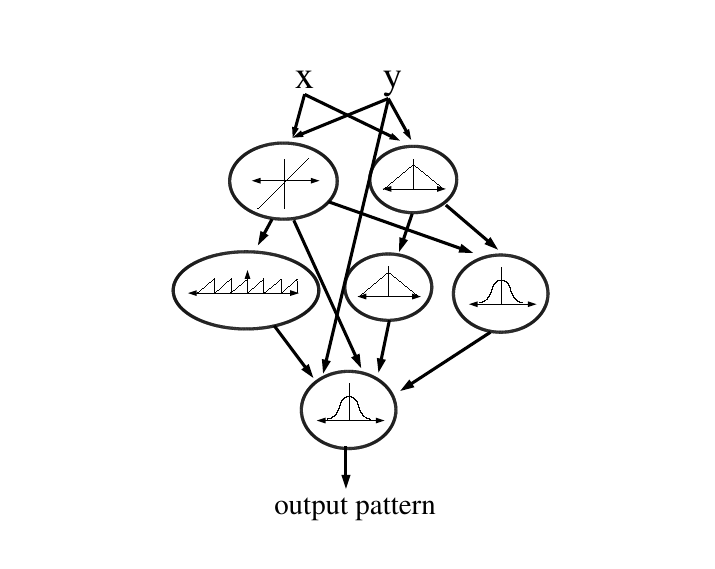
\includegraphics[scale=0.25]{../Figures/Misc/cppnNetwork.png}
\end{center}
\end{figure}
\item Produce symmetrical and repetitive patterns
\item Appropriate for problems with geometrical structure
\end{itemize}
\end{frame}


\begin{frame}{NeuroEvolution through Augmented Topologies (NEAT)~\cite{stanley2002evolving}}
\begin{block}{Some key points of this method are:}
\begin{itemize}
\item Evolving neural network topologies along with weights
\item Crossover between different topologies
\item Structural innovation through speciation (New species have time to improve)
\end{itemize}
\end{block}
\end{frame}


\begin{frame}{Novelty Search}
\putat{230}{-170}{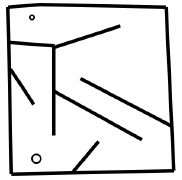
\includegraphics[scale=0.5]{../Figures/Misc/noveltyMaze.png}}
\begin{block}{What is novelty search:}
\begin{itemize}
\item Traditionally fitness measures how good an individual is (Objective function).
\item Objective function can prevent evolution reaching the global maximum.
\item Abandon the objective.
\item Try finding novelty in behavior space.
\item Random?
\end{itemize}
\end{block}
\begin{definition}[Sparsity]
\begin{equation*}
s(x) = \cfrac{1}{k} \sum_{i=0}^k dist(x, b_i)
\end{equation*}
\end{definition}
\end{frame}



\section{Research Question}

\begin{frame}{Research Topics}
\begin{itemize}
\item Gravity
\begin{itemize}
\item Performance under different conditions of gravity
\end{itemize}
\item Novelty search
\begin{itemize}
\item Performance, in respect to the original fitness
\item Performance, in behavior space
\item Behavior, what is a good behavior metric?
\end{itemize}
\item Other evolutionary algorithms
\begin{itemize}
\item Genetic algorithm with direct coding
\item Random generative encoding
\item Covariance Matrix Adaptation Evolution Strategy (CMA-ES)
\item Differential Evolution (jDE)
\end{itemize}
\item Can we evolve CPPNs with other evolutionary algorithms?
\end{itemize}
\end{frame}





\section{Approach}

\begin{frame}{Things completed so far\ldots}
\begin{itemize}
%\item All tools documented
\item Replication of the results from~\cite{cheney2013unshackling}
\item Generative random encoding
\item Simple genetic algorithm
\item Implementation of CPPN-NEAT experiment (HyperNEAT~C++~library)
\item Novelty search
\item Competition between species (novelty, fitness)
\item Combination of novelty and fitness
\end{itemize}
\end{frame}




\begin{frame}{Random Soft Robots}
\begin{block}{Random}
Assign materials to voxels randomly.
\end{block}
\begin{block}{Generative encoding}
Only two parameters can change in this encoding.
\begin{enumerate}
\item The probability of adding a new voxel into the structure.
\item The probability that the new voxel introduced will use the same kind of material as its connection.
\end{enumerate}
\end{block}
\begin{block}{Random CPPNs}
Evolution with high mutation power and no fitness information.
\end{block}
\end{frame}

\begin{frame}{Simple genetic algorithm}
\begin{itemize}
\item GAlib C++ library
\item Each genome is represented by a stream of real numbers in $[ 0,1 ]$.
\item The length of this stream is equal to:
\begin{equation*}
l = n \times (m + 1)
\end{equation*}
, where $n$, is the number of total voxels and $m$ is the number of materials.
\item For a lattice's dimensions of $10 \times 10 \times 10$ and $4$ materials the length of the genome is $5000$.
\item Simple genetic algorithm fails to produce locomotion.
\item No structure knowledge.
\end{itemize}
\end{frame}


\begin{frame}{CPPN-NEAT}
\begin{itemize}
\item HyperNEAT C++
\item Each genome is represented by a CPPN.
\item This CPPN is queried for each input coordinate to output the existance and the type of the material.
\item NEAT evolves these CPPNs.
\item In each generation, speciation. Population is split into species, new species can survive easier than old.
\end{itemize}
\end{frame}


\begin{frame}{CPPN-NEAT with Novelty Search~\cite{lehman2011abandoning}}
\begin{itemize}
\item Same code base
\item Novelty takes the place of fitness
\item Novel individuals stored in a list
\item For each new individual in the population, check its novelty in respect to the stored novel individuals.
\begin{itemize}
\item Sparsity
\end{itemize}
\end{itemize}
\end{frame}

\begin{frame}{Behavior}
How can we go from fitness to behavior:\\
\vspace{0.2cm}
\begin{center}
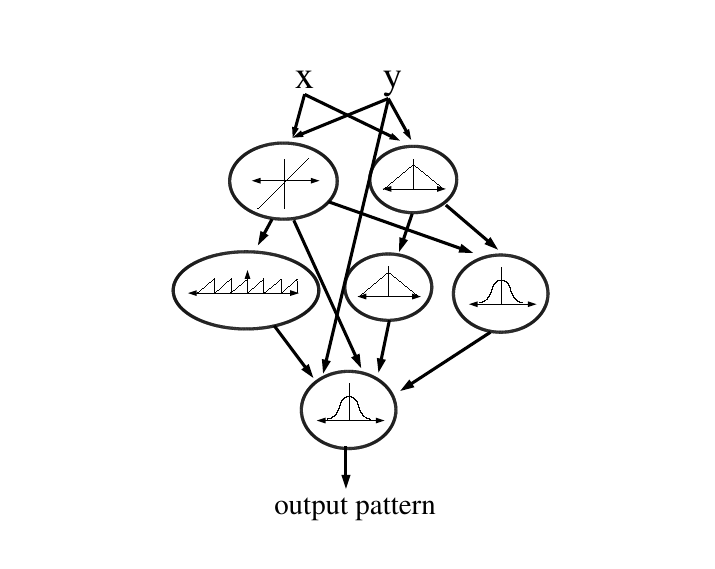
\includegraphics[height=0.15\textheight]{../Figures/Misc/cppnNetwork.png}\	
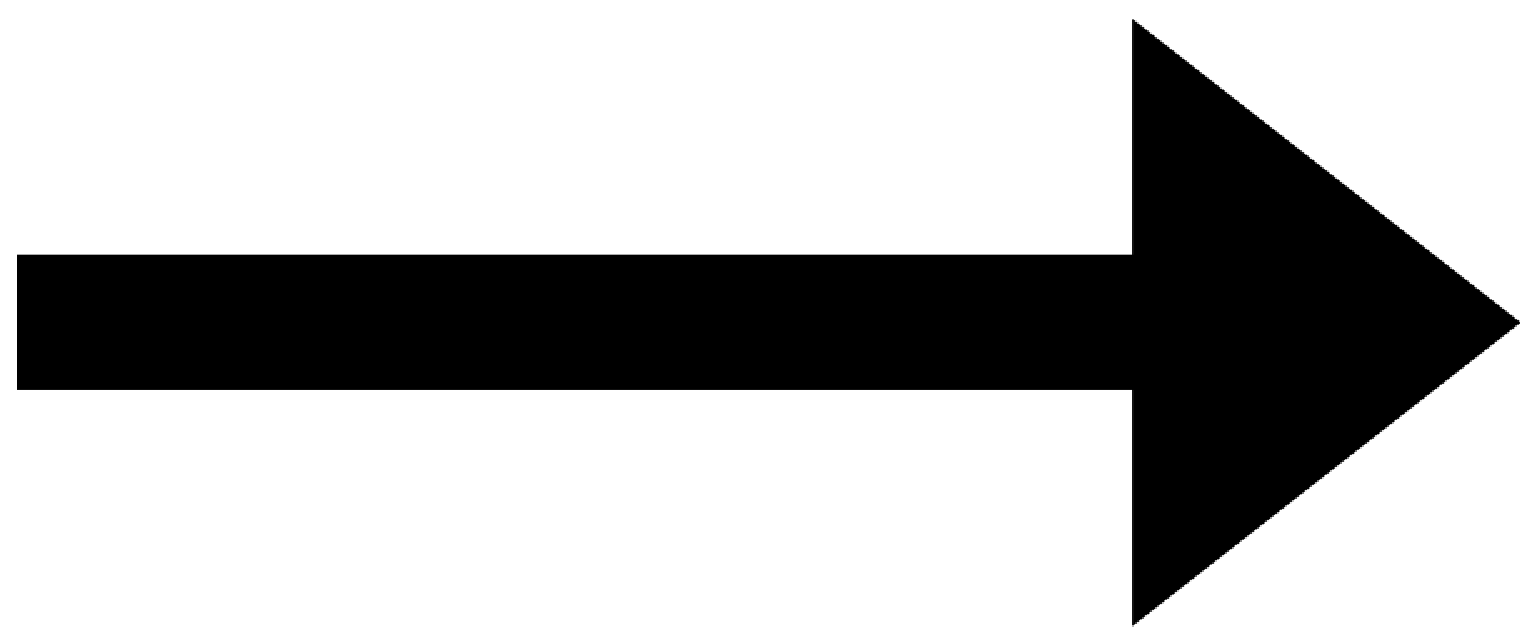
\includegraphics[height=0.05\textheight]{../Figures/Misc/Arrow_east.eps}\	
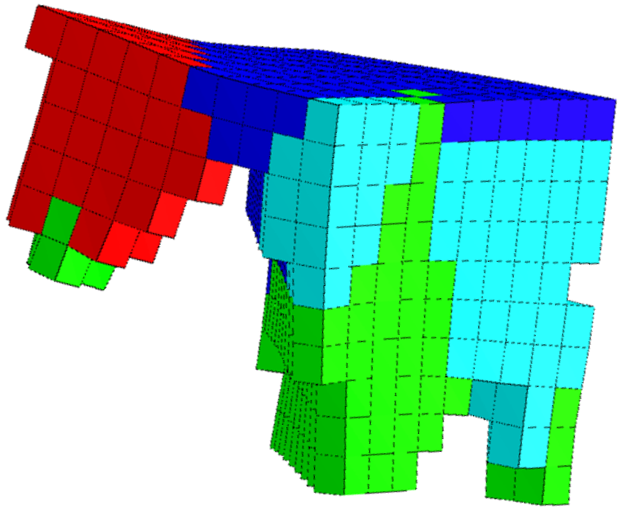
\includegraphics[height=0.15\textheight]{../Figures/Misc/unshacklingEvolutionFigure2.png}\	
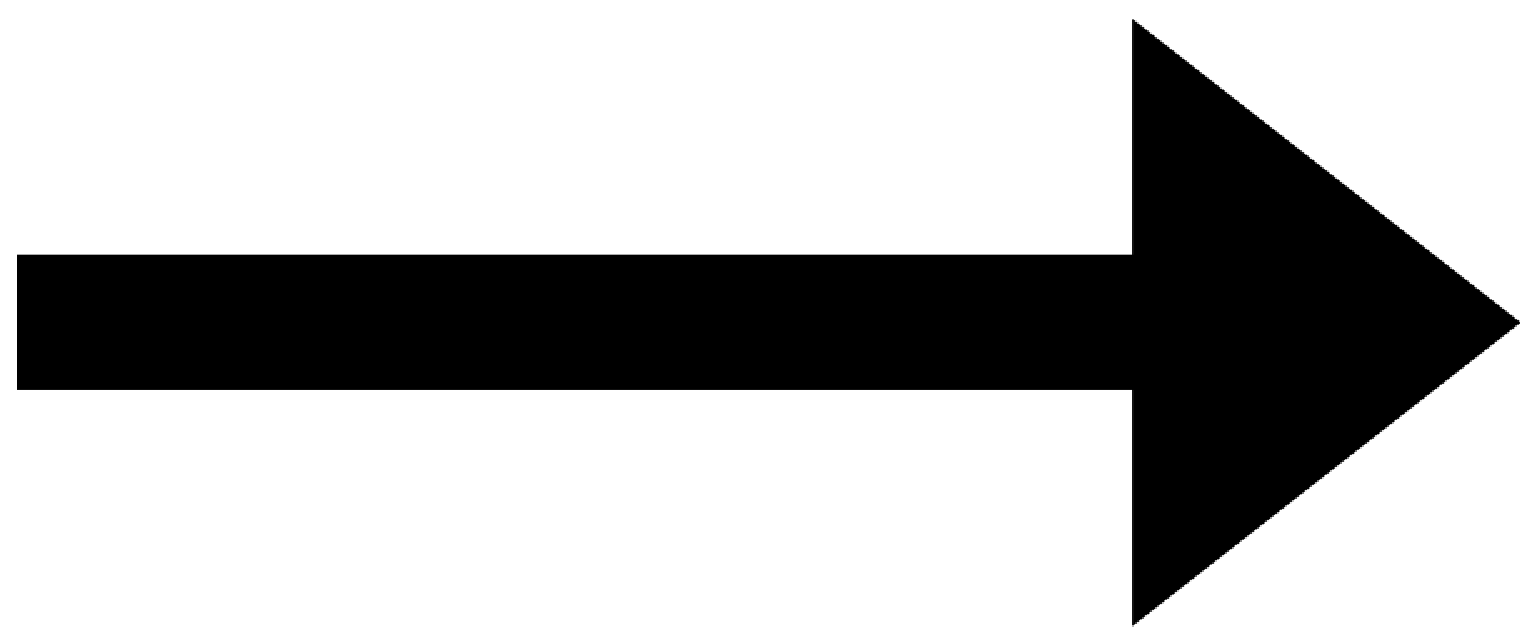
\includegraphics[height=0.05\textheight]{../Figures/Misc/Arrow_east.eps}\	
{\huge $F(x)$ }\	
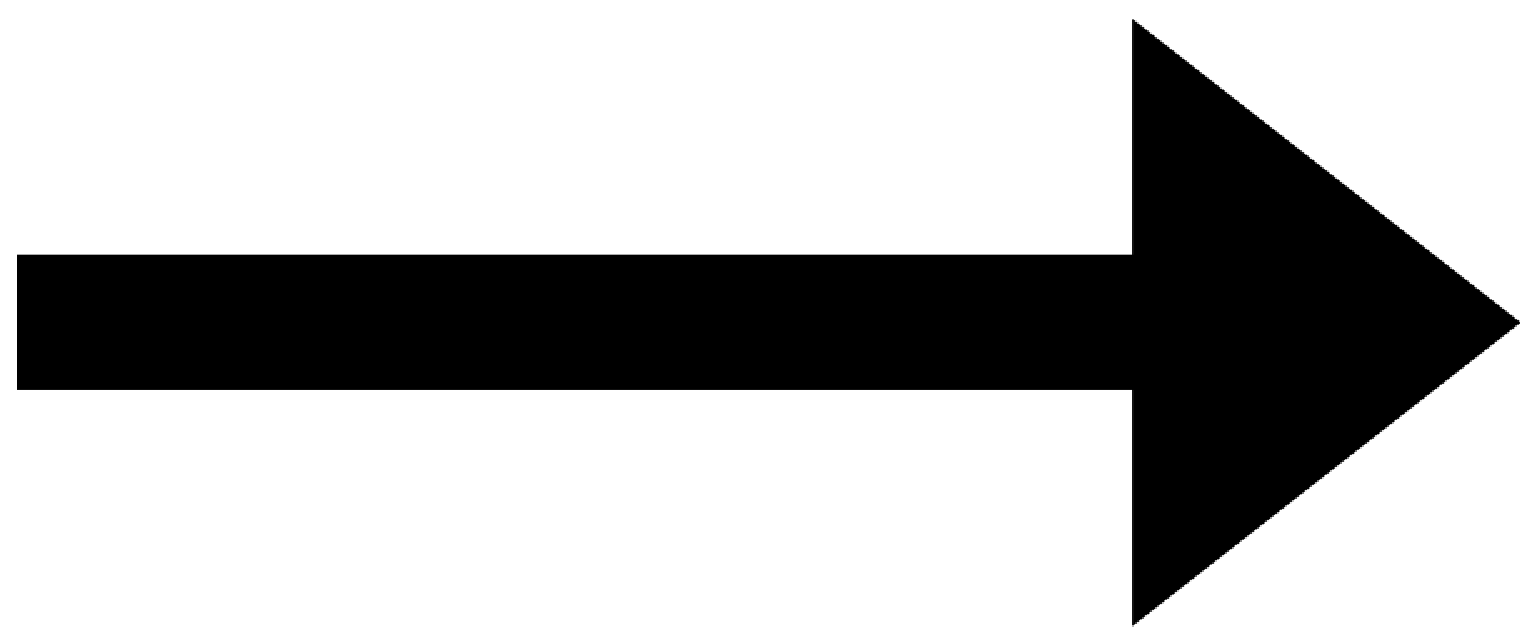
\includegraphics[height=0.05\textheight]{../Figures/Misc/Arrow_east.eps}\	
{\huge $B(x)$ }\\
\end{center}
\vspace{0.10cm}
Examples:\\
\begin{center}
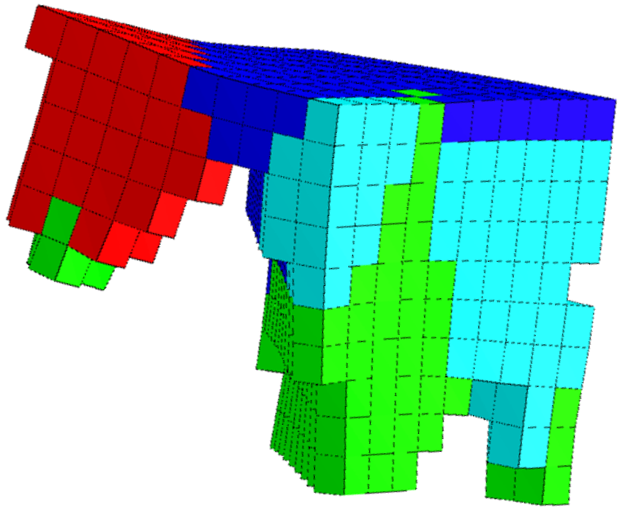
\includegraphics[height=0.15\textheight]{../Figures/Misc/unshacklingEvolutionFigure2.png}\	
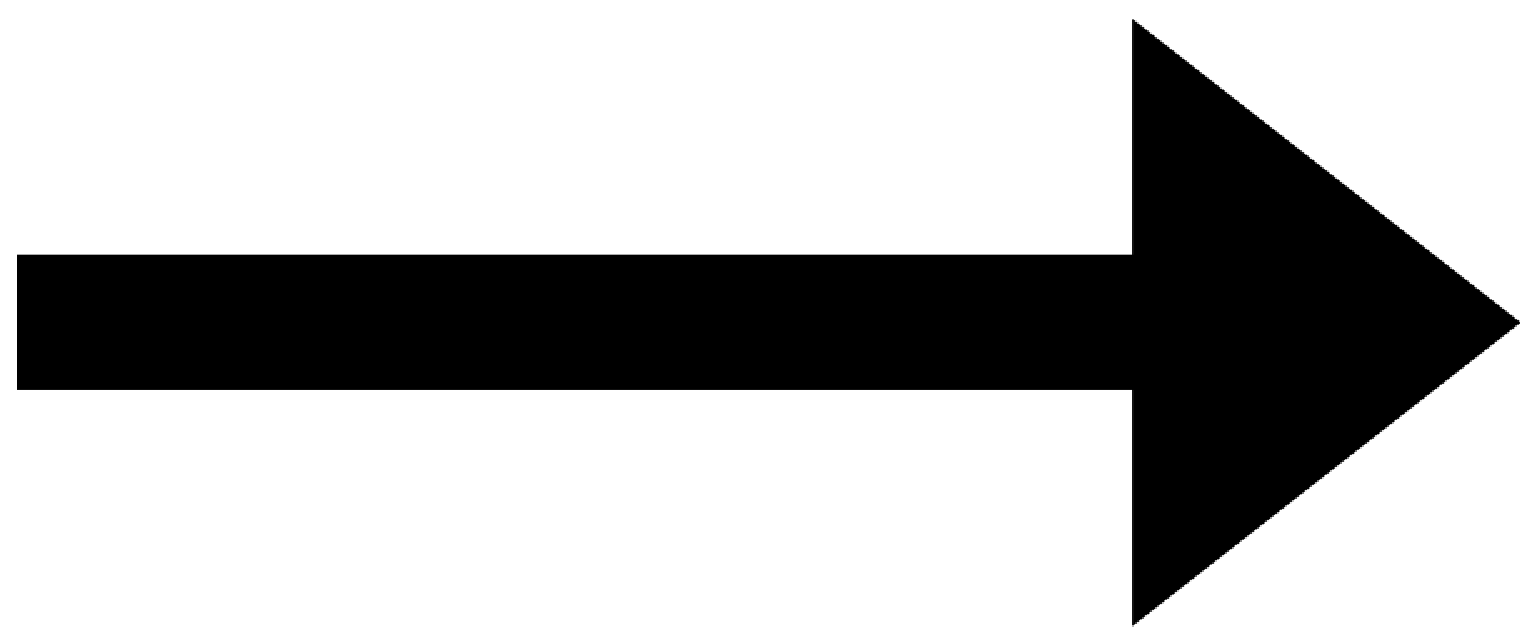
\includegraphics[height=0.05\textheight]{../Figures/Misc/Arrow_east.eps}\	
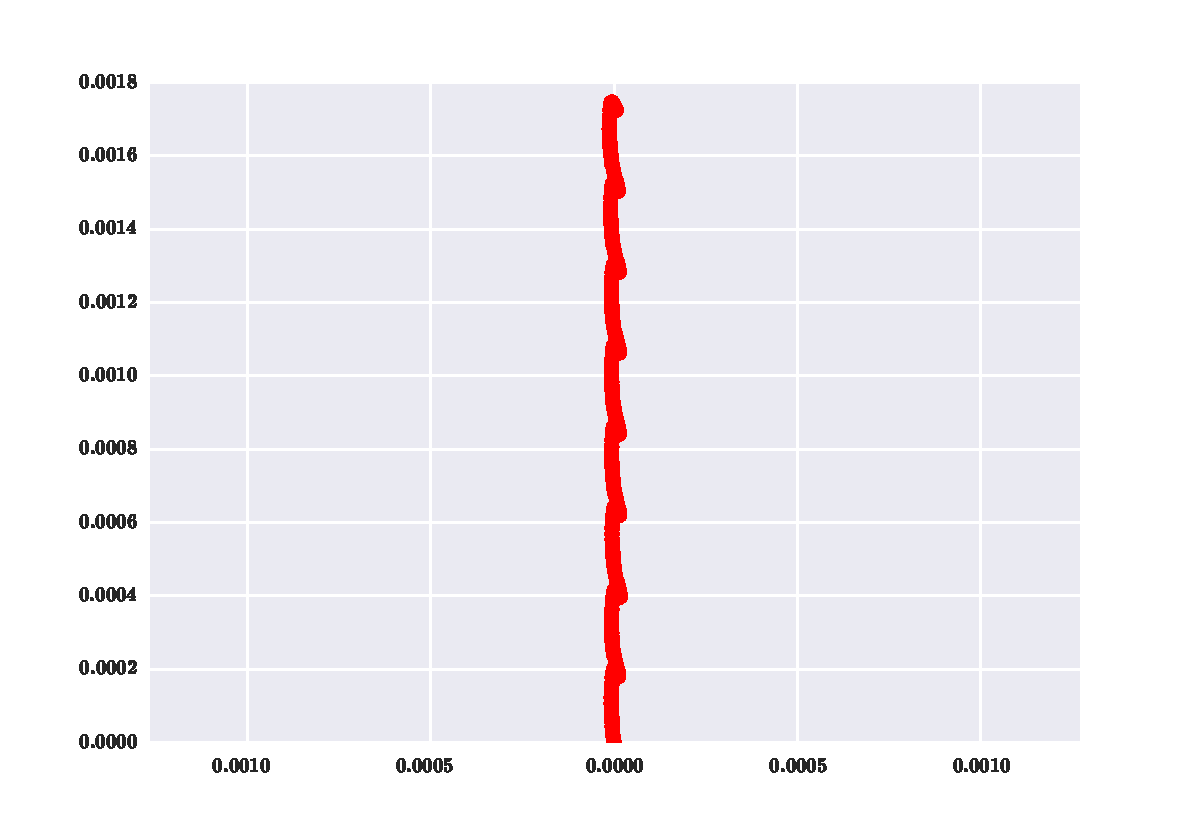
\includegraphics[height=0.15\textwidth]{../Figures/Behaviors/03.pdf}
\\
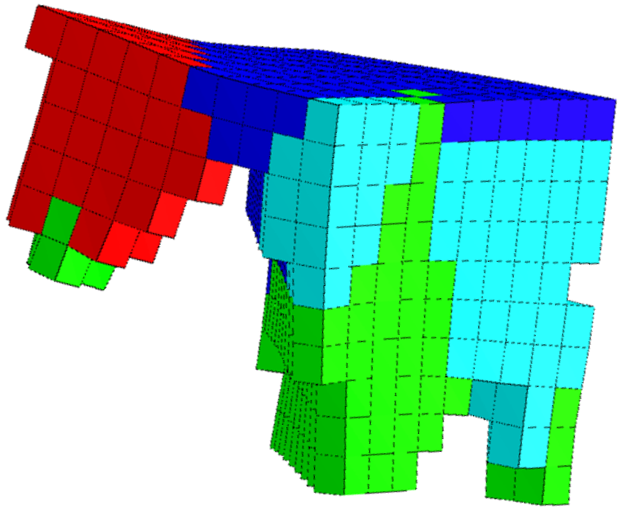
\includegraphics[height=0.15\textheight]{../Figures/Misc/unshacklingEvolutionFigure2.png}\	
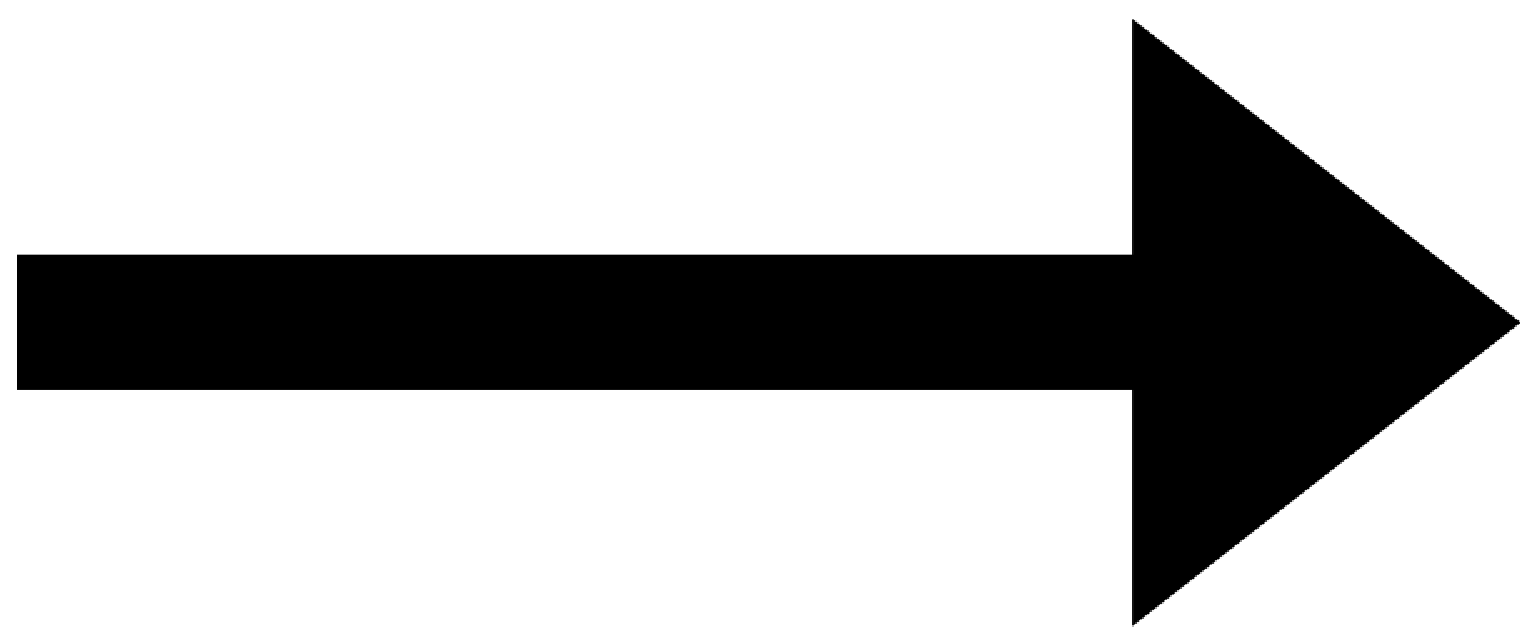
\includegraphics[height=0.05\textheight]{../Figures/Misc/Arrow_east.eps}\	
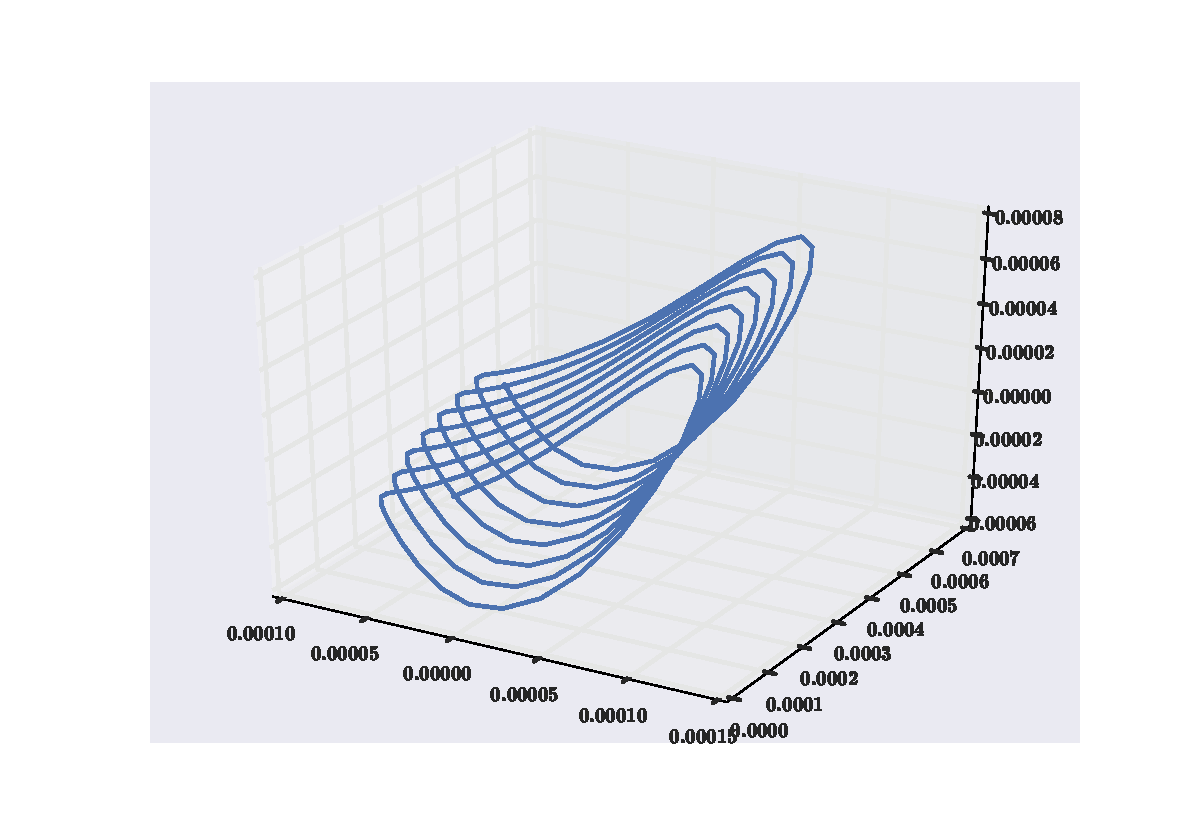
\includegraphics[height=0.15\textwidth]{../Figures/Behaviors/11.pdf}
\\
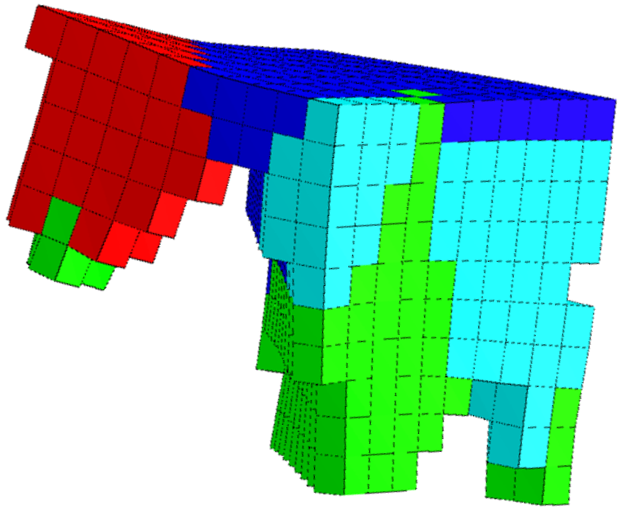
\includegraphics[height=0.15\textheight]{../Figures/Misc/unshacklingEvolutionFigure2.png}\	
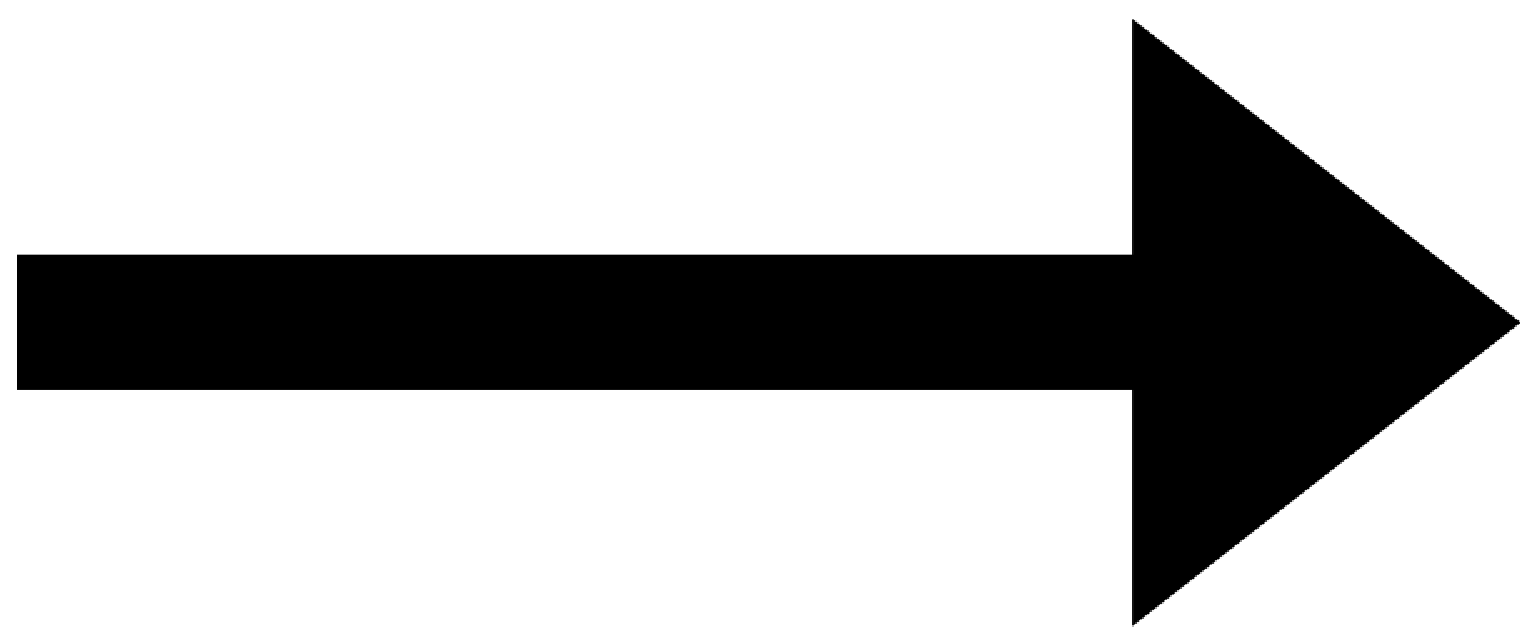
\includegraphics[height=0.05\textheight]{../Figures/Misc/Arrow_east.eps}\	
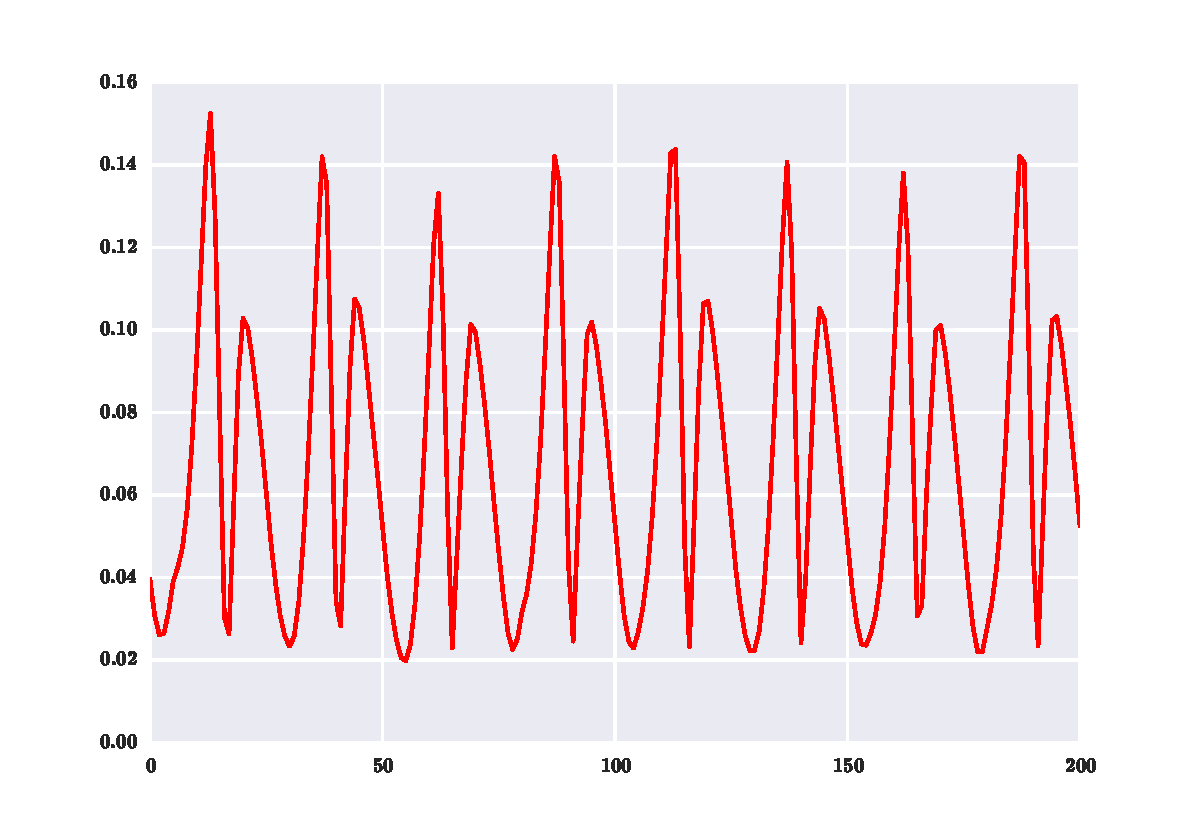
\includegraphics[height=0.15\textwidth]{../Figures/Behaviors/22.pdf}
\end{center}
\end{frame}


\begin{frame}{Behavior}
\begin{block}{Behavior types can be used:}
\begin{itemize}
\item Trajectory 3D, 2D
\item Pace
\item Voxels touching ground
\item Kinetic energy
\item Maximum pressure
\end{itemize}
\end{block}
\begin{block}{Behavior similarity can be computed:}
\begin{itemize}
\item Sum of Euclidean distances per timestep
\item Cross-correlation
\end{itemize}
\end{block}
\end{frame}

\begin{frame}[allowframebreaks]{Behavior Examples}

\begin{minipage}{\textwidth}
\begin{block}{2D - Trajectories:}
\begin{center}
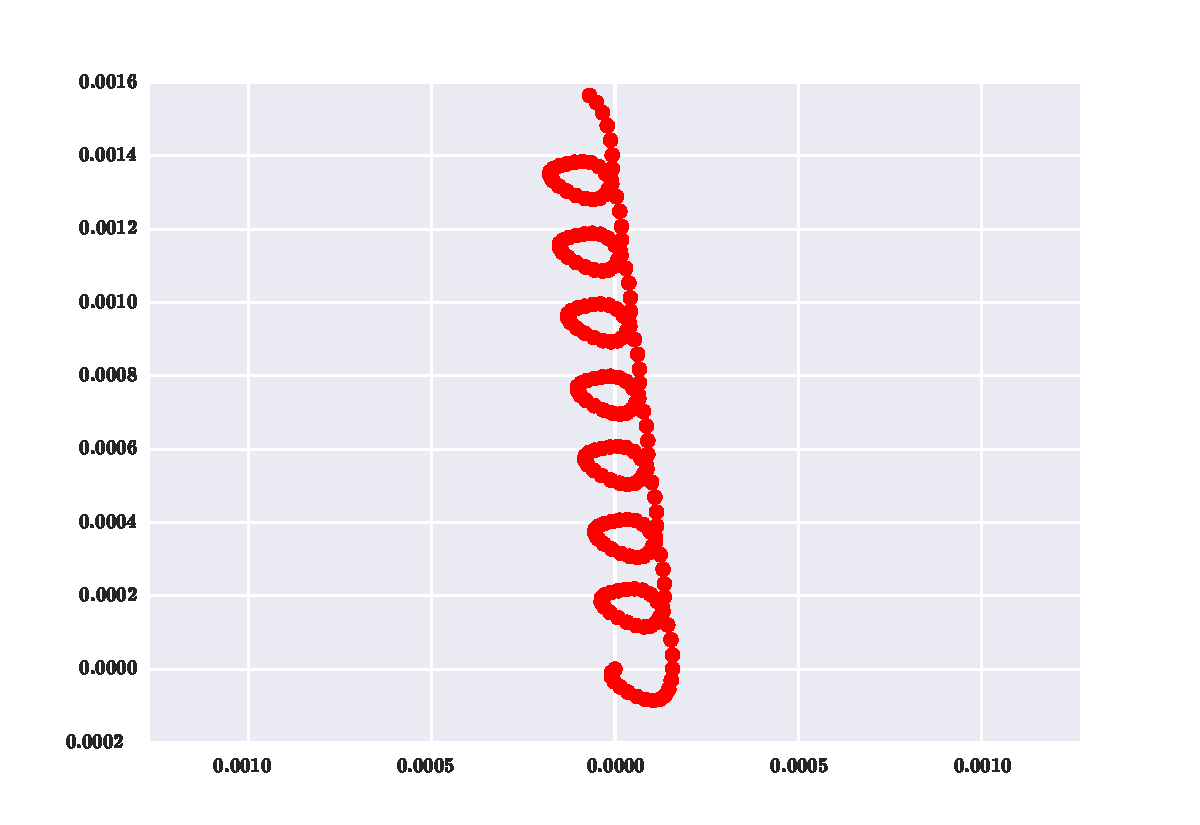
\includegraphics[width=0.25\textwidth]{../Figures/Behaviors/00.pdf}
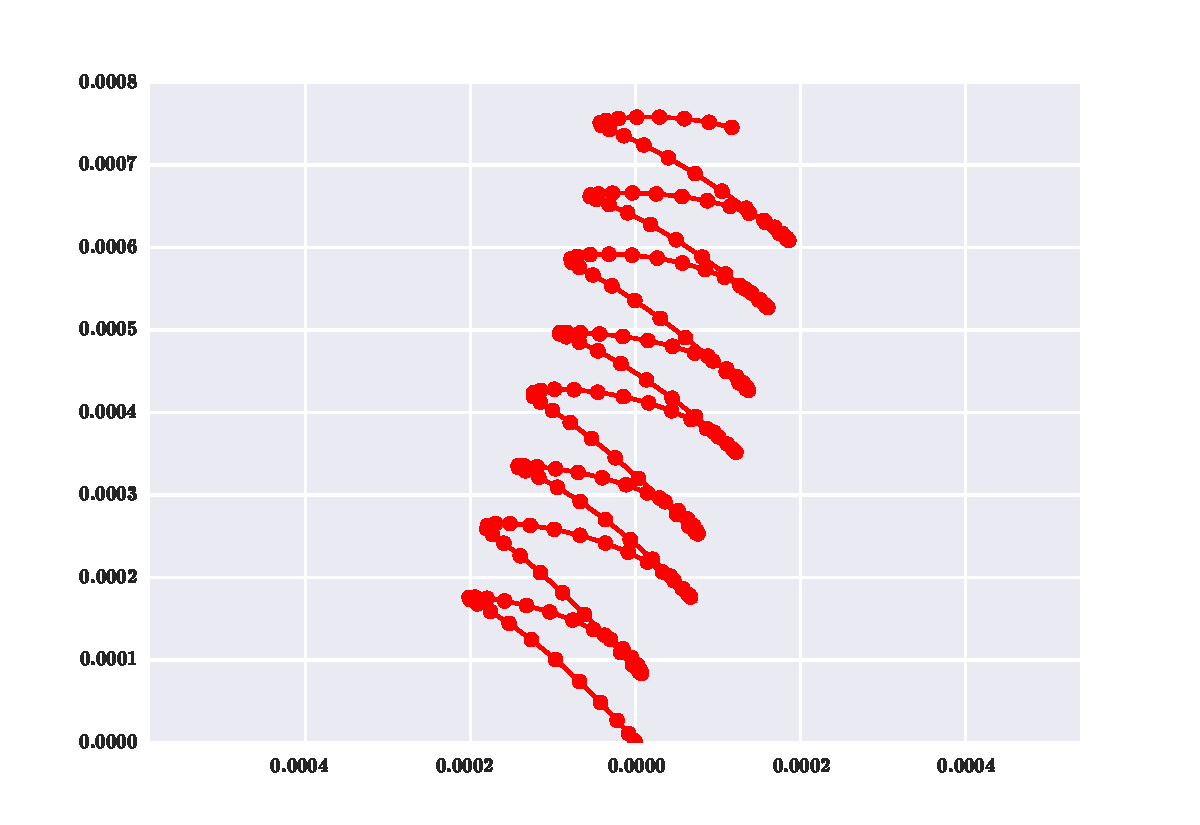
\includegraphics[width=0.25\textwidth]{../Figures/Behaviors/01.pdf}
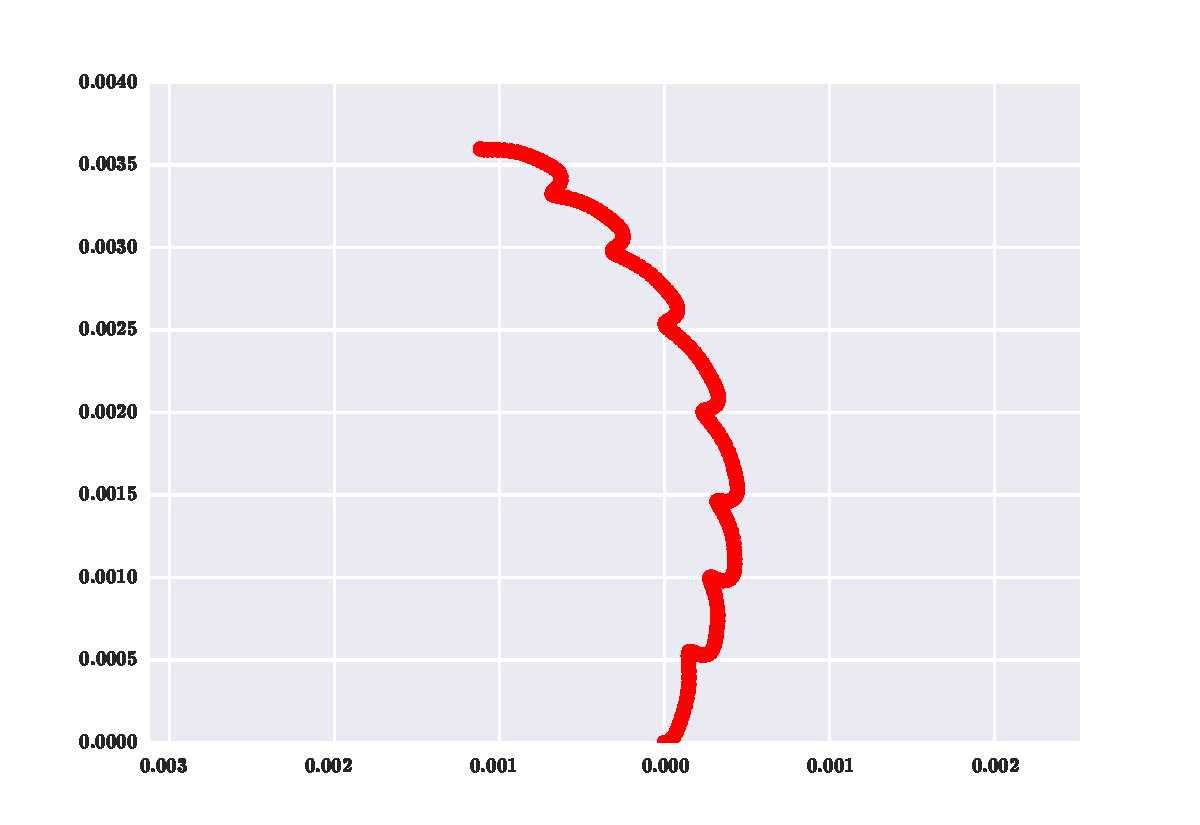
\includegraphics[width=0.25\textwidth]{../Figures/Behaviors/02.pdf}
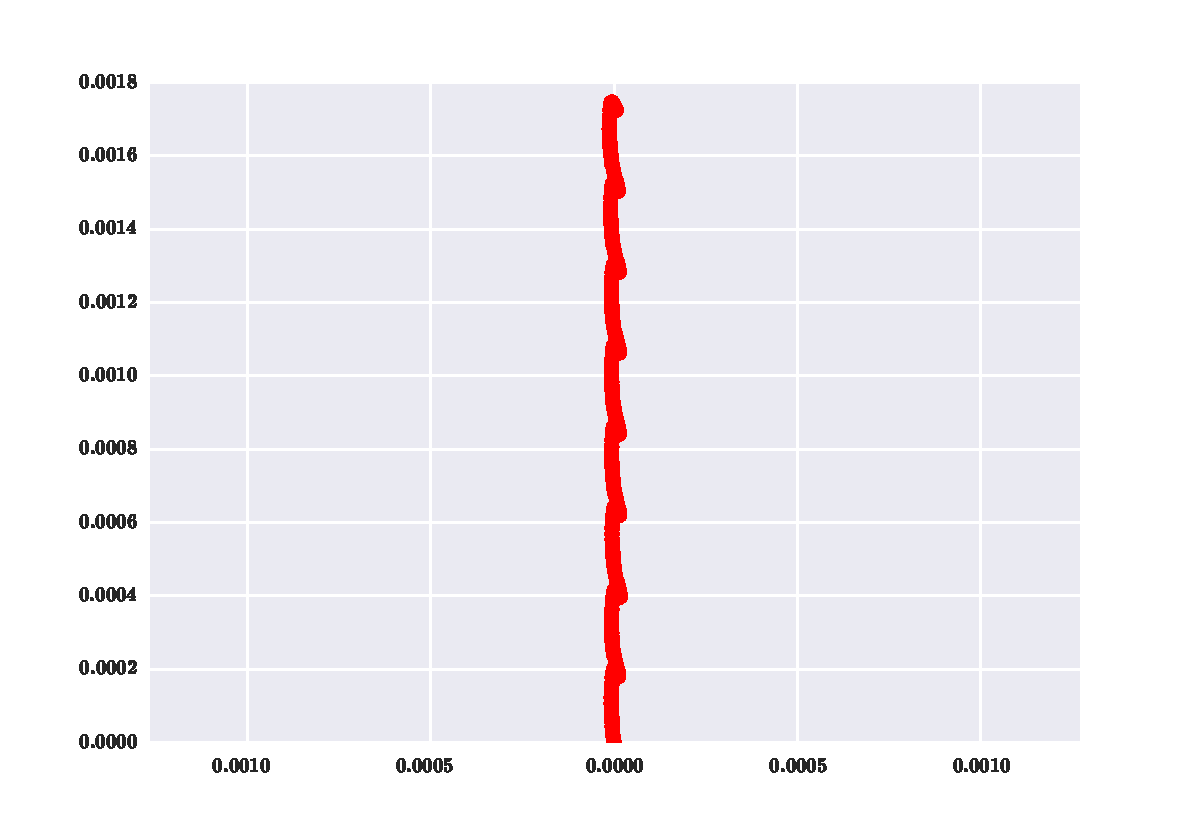
\includegraphics[width=0.25\textwidth]{../Figures/Behaviors/03.pdf}
\end{center}
\end{block}
\begin{block}{3D - Trajectories}
\begin{center}
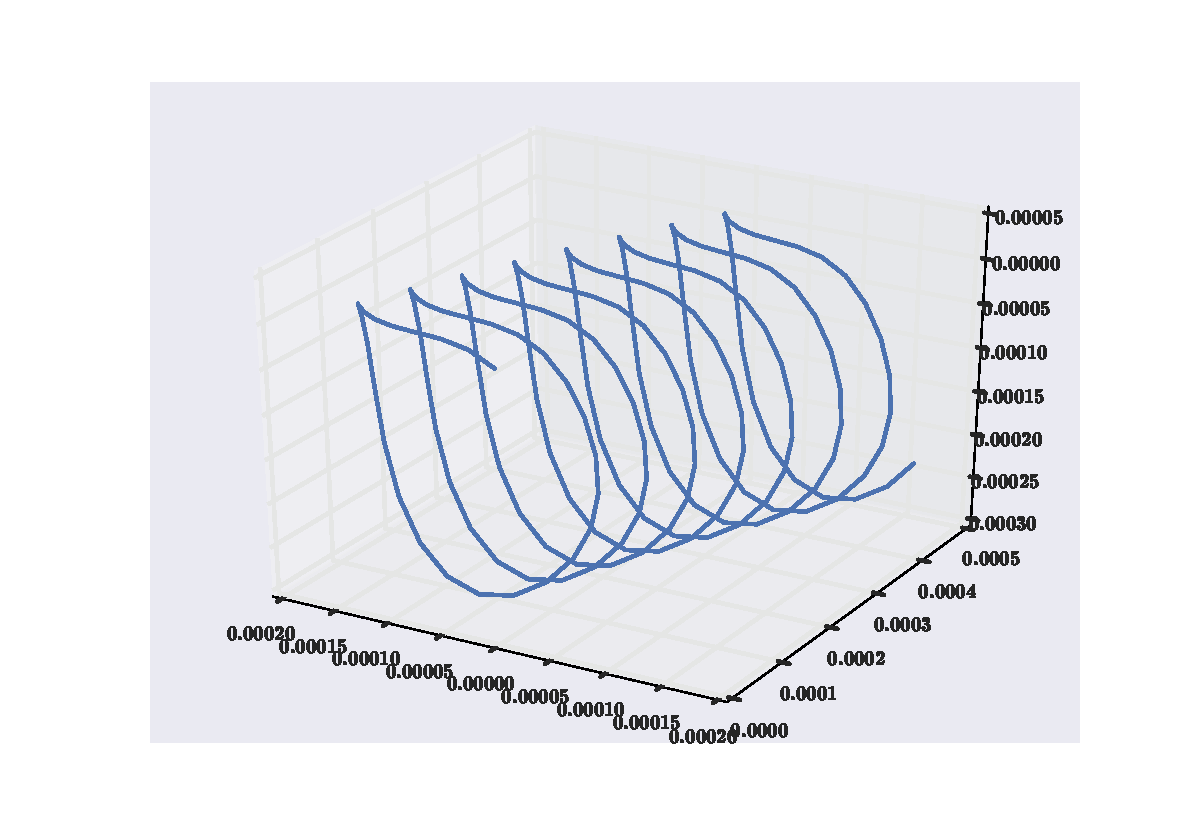
\includegraphics[width=0.25\textwidth]{../Figures/Behaviors/10.pdf}
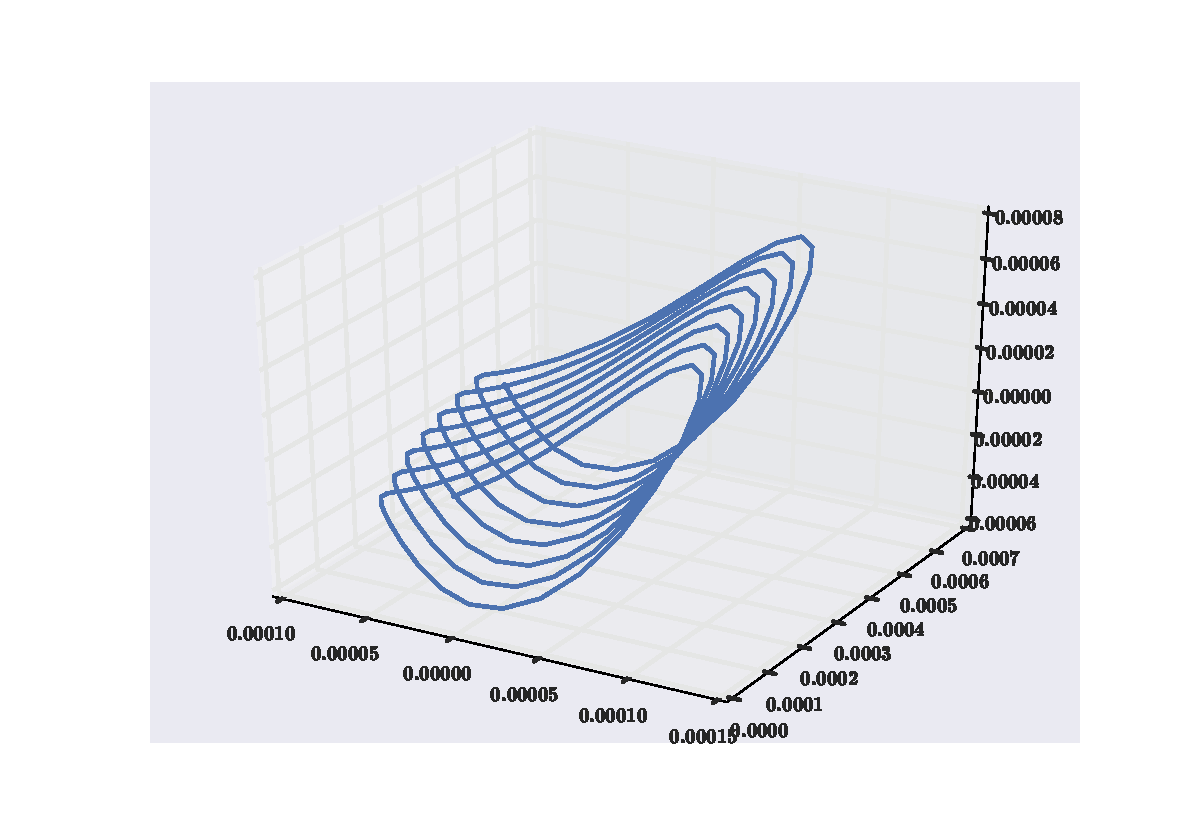
\includegraphics[width=0.25\textwidth]{../Figures/Behaviors/11.pdf}
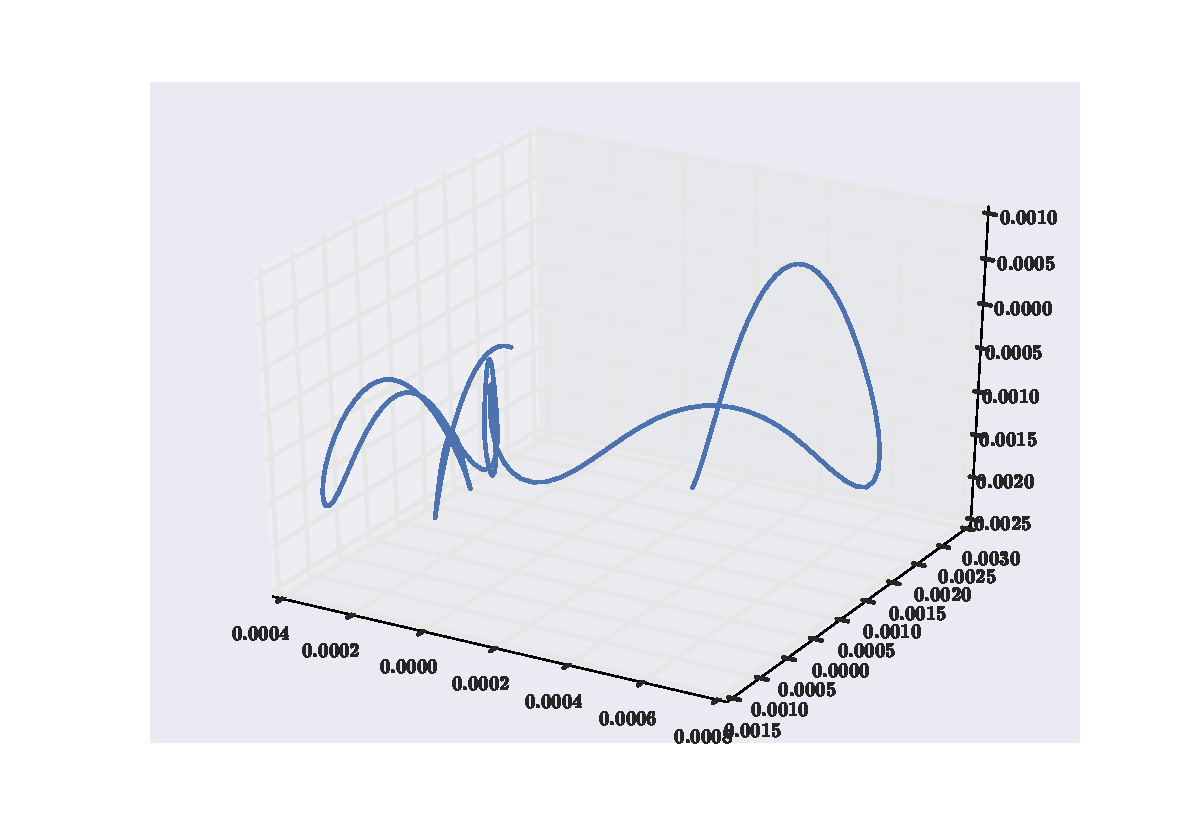
\includegraphics[width=0.25\textwidth]{../Figures/Behaviors/12.pdf}
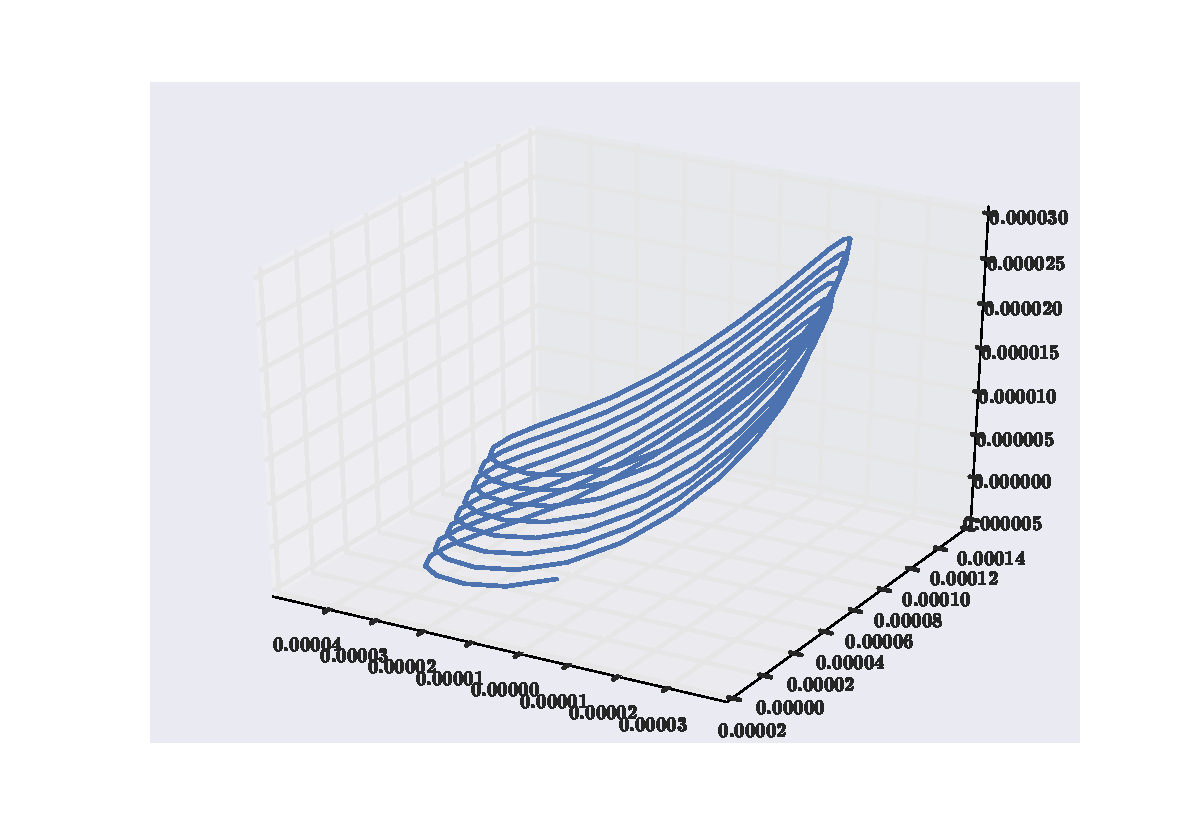
\includegraphics[width=0.25\textwidth]{../Figures/Behaviors/13.pdf}
\end{center}
\end{block}
\end{minipage}

\begin{minipage}{\textwidth}
\begin{block}{Pace per timestep}
\begin{center}
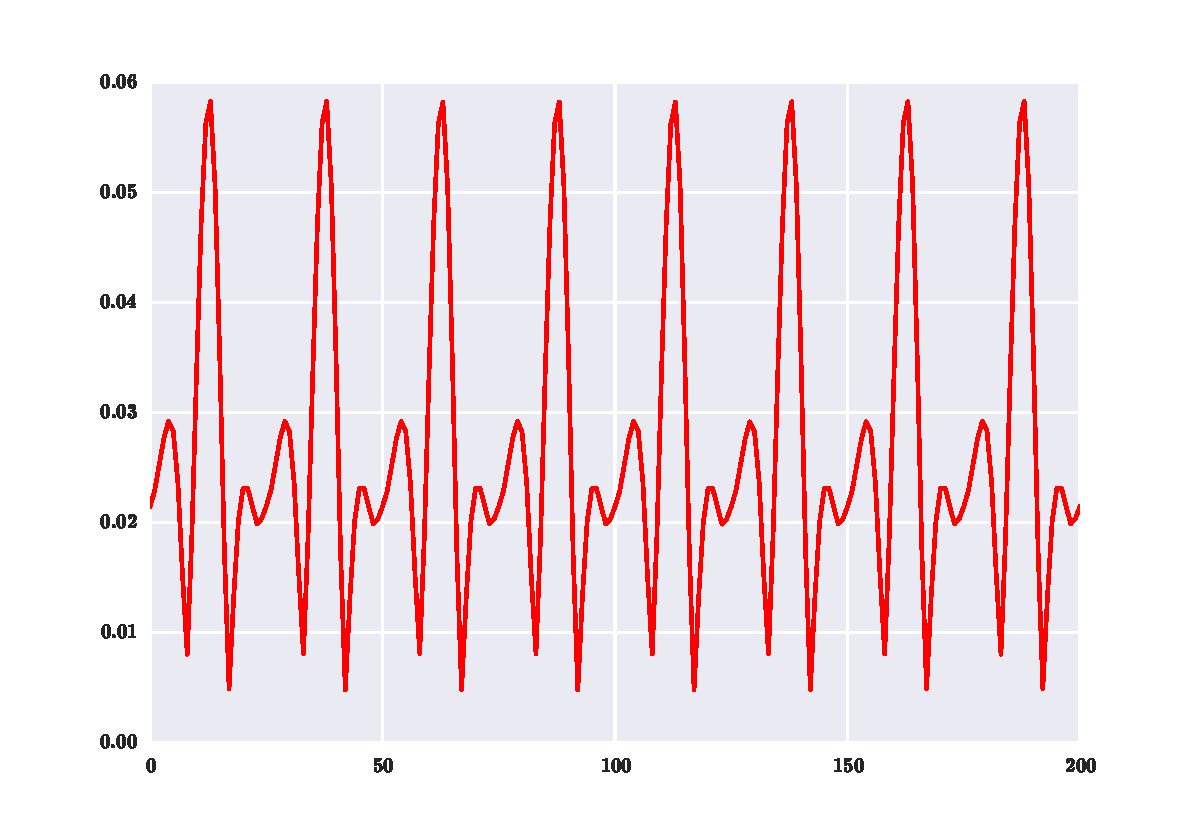
\includegraphics[width=0.25\textwidth]{../Figures/Behaviors/20.pdf}
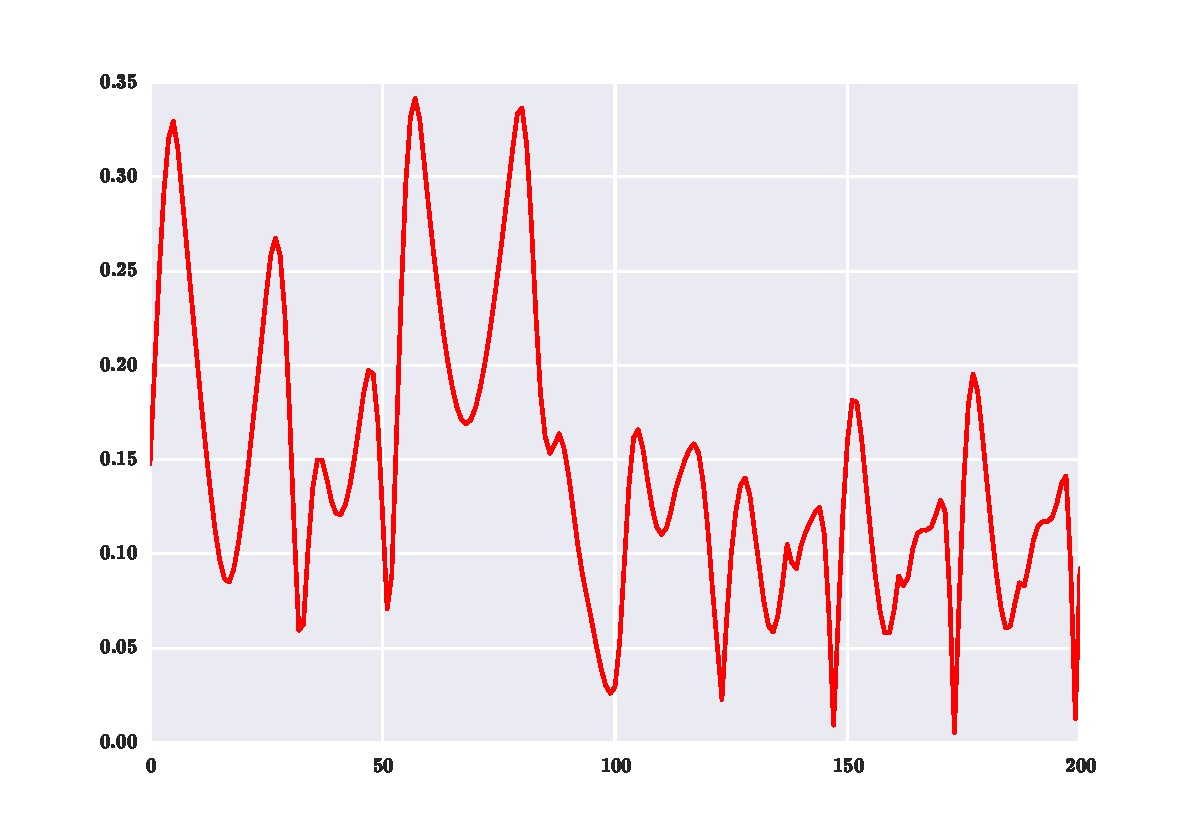
\includegraphics[width=0.25\textwidth]{../Figures/Behaviors/21.pdf}
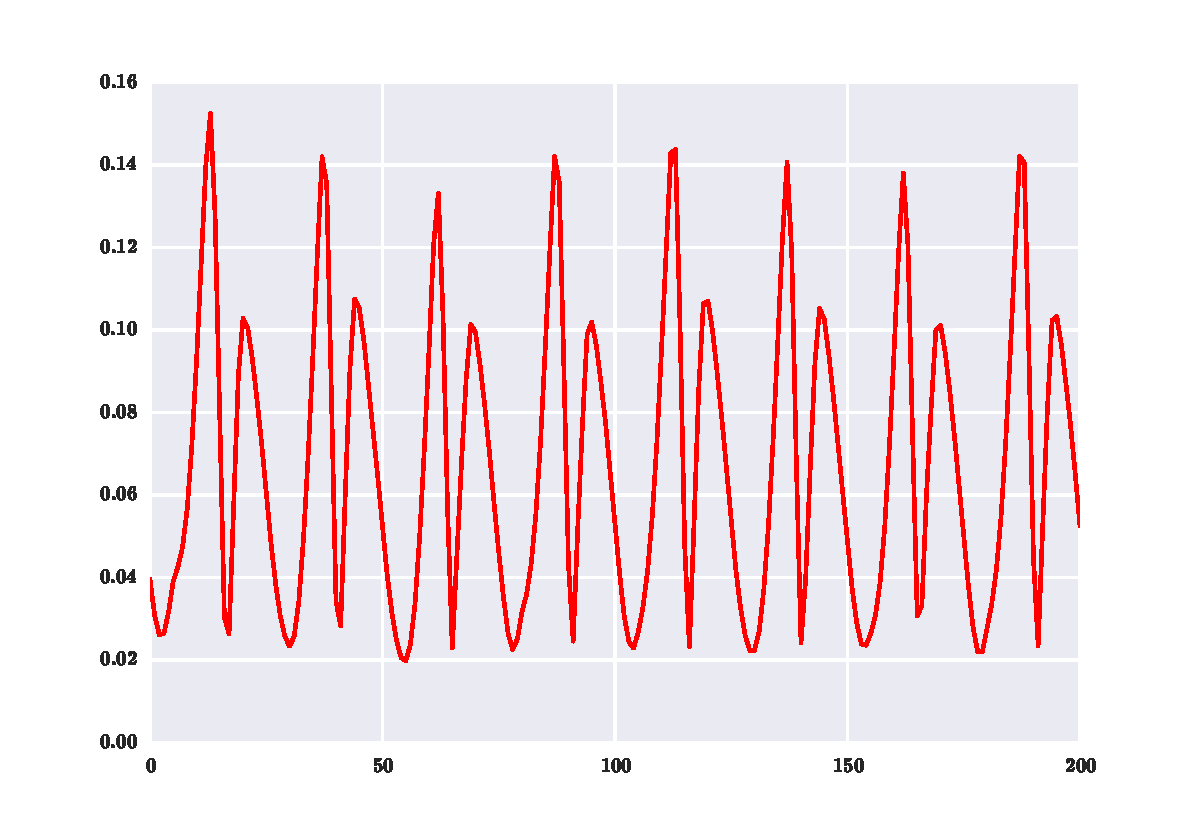
\includegraphics[width=0.25\textwidth]{../Figures/Behaviors/22.pdf}
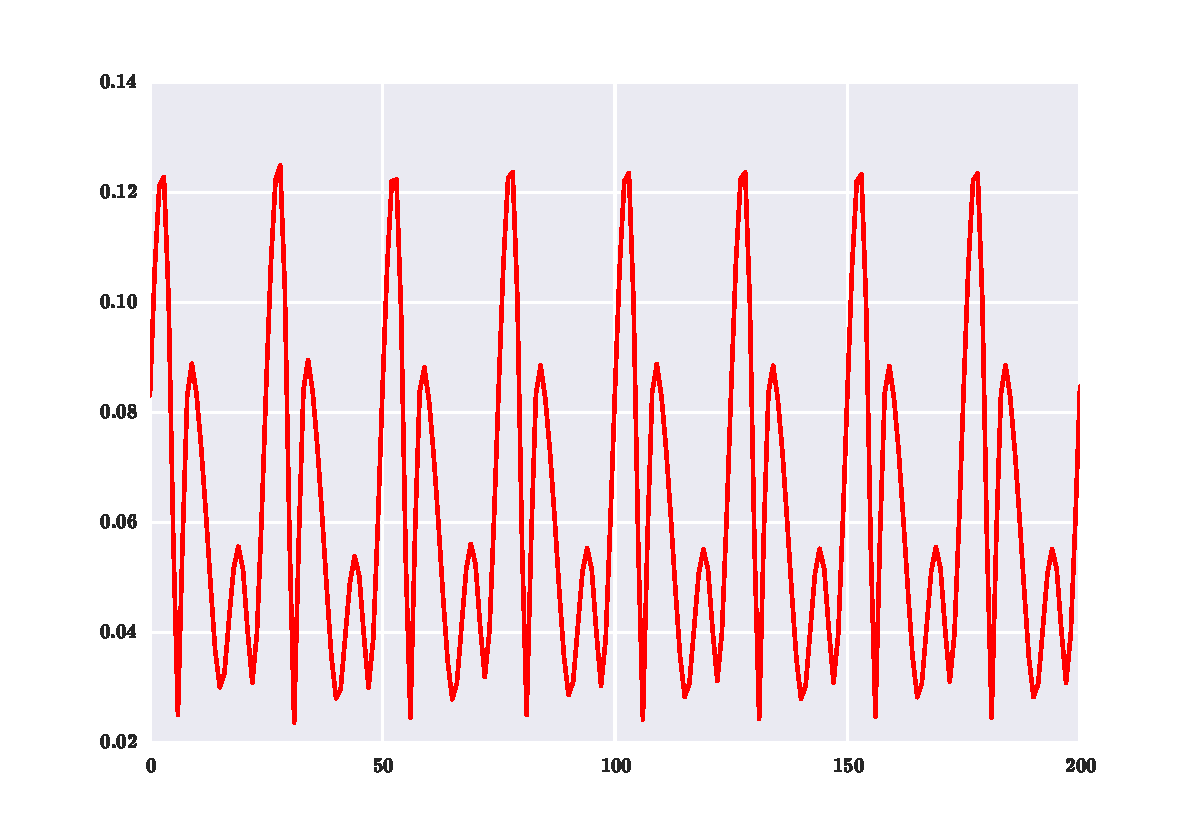
\includegraphics[width=0.25\textwidth]{../Figures/Behaviors/23.pdf}
\end{center}
\end{block}
\begin{block}{Pace - DFT}
\begin{center}
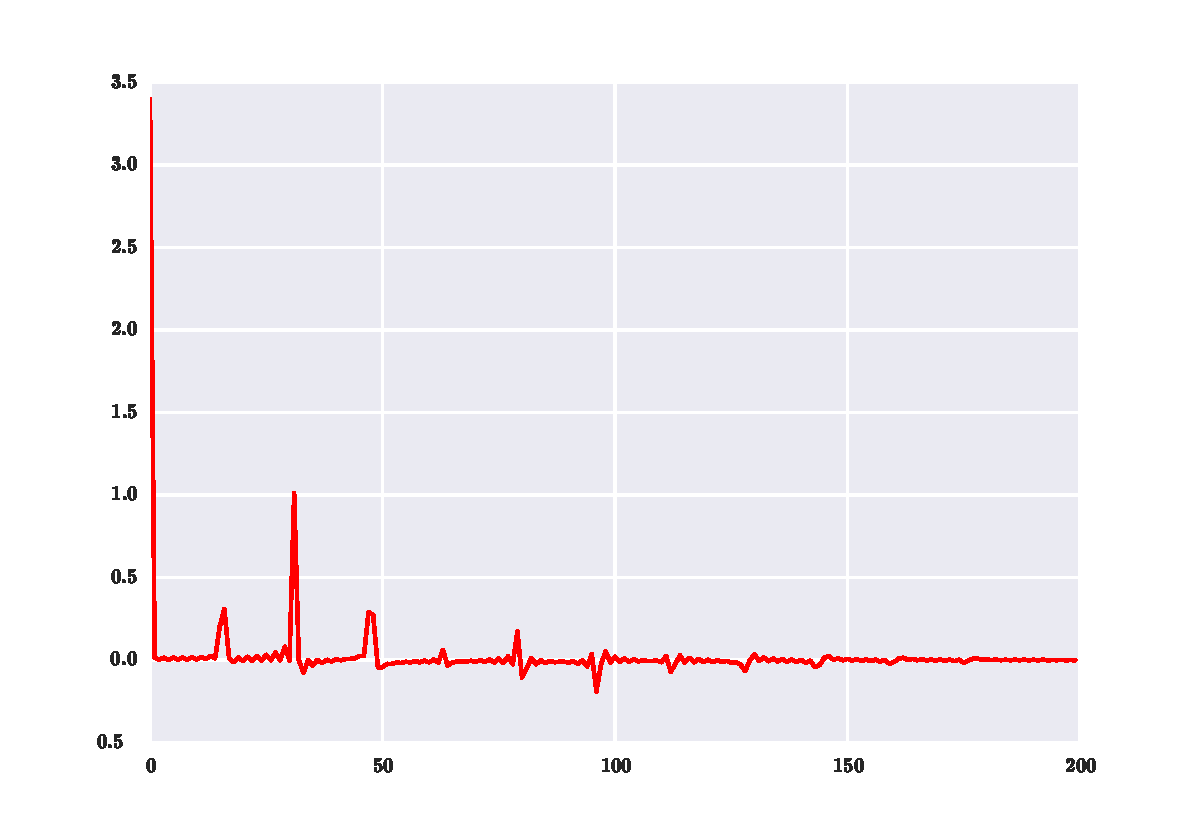
\includegraphics[width=0.25\textwidth]{../Figures/Behaviors/30.pdf}
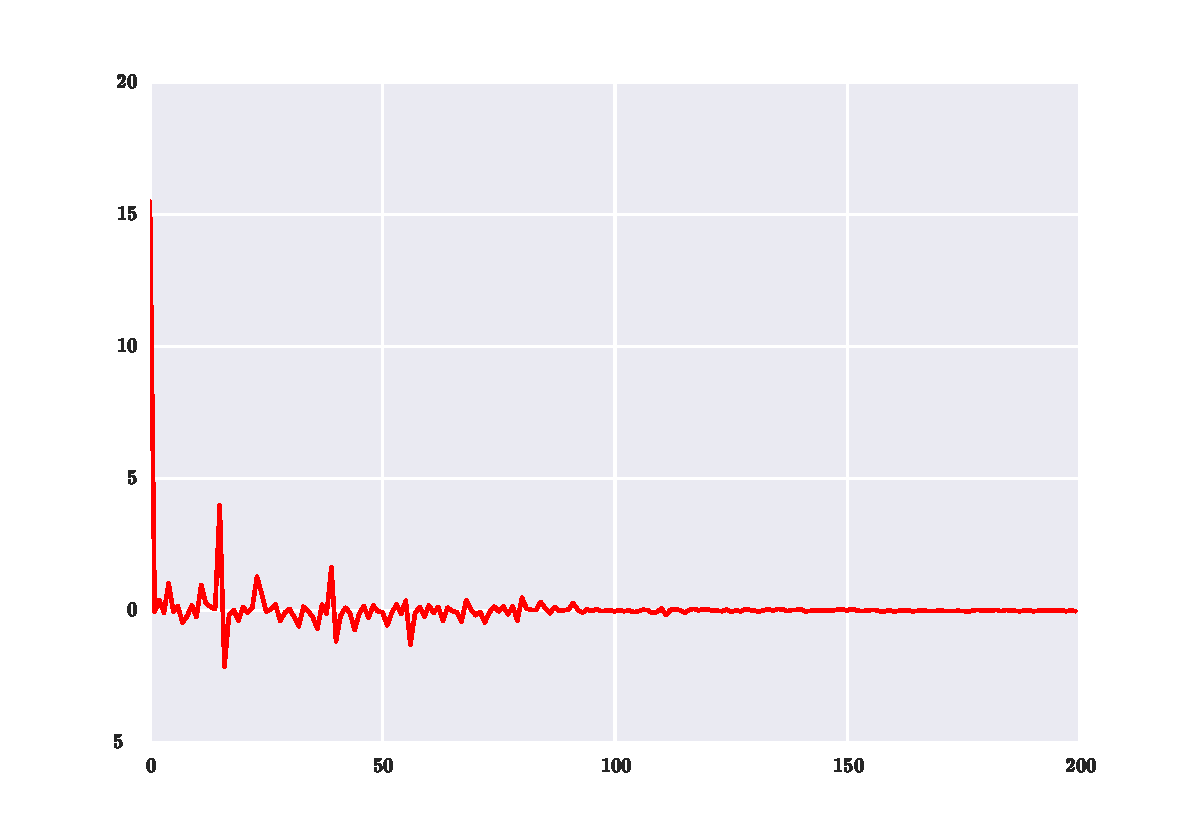
\includegraphics[width=0.25\textwidth]{../Figures/Behaviors/31.pdf}
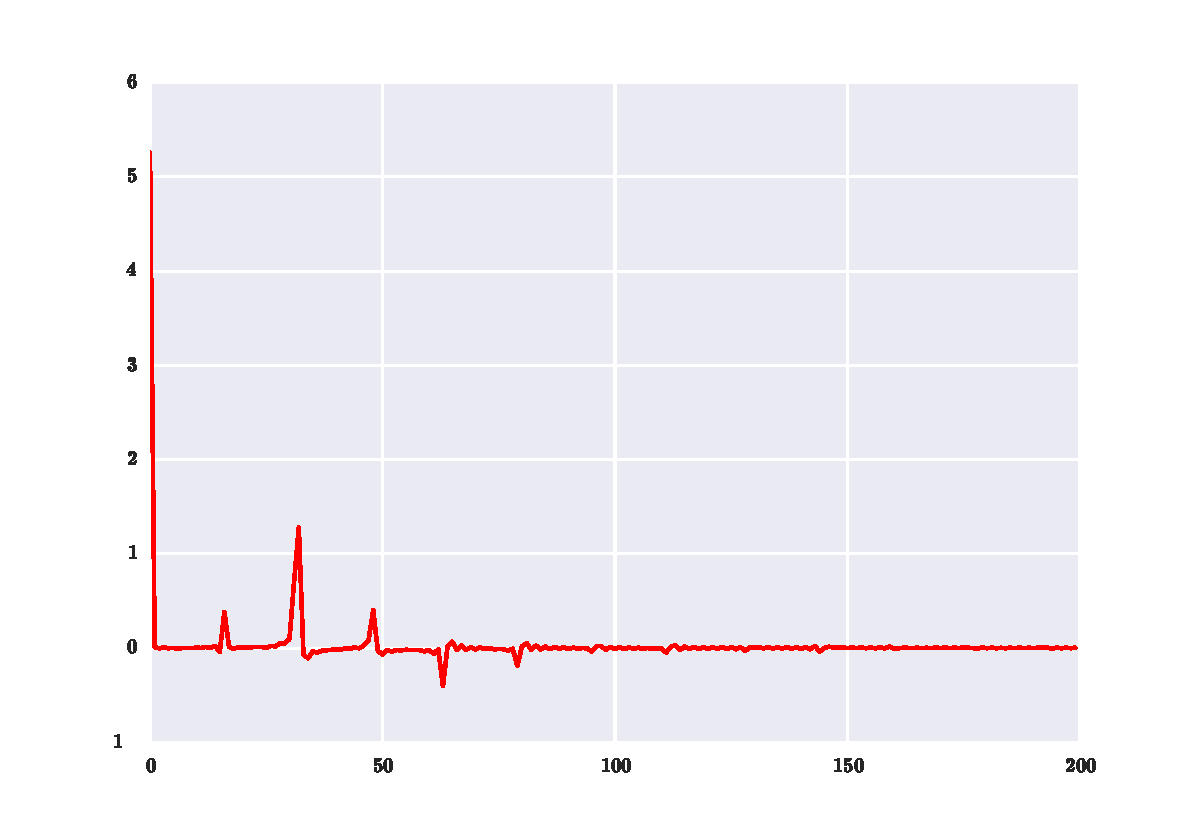
\includegraphics[width=0.25\textwidth]{../Figures/Behaviors/32.pdf}
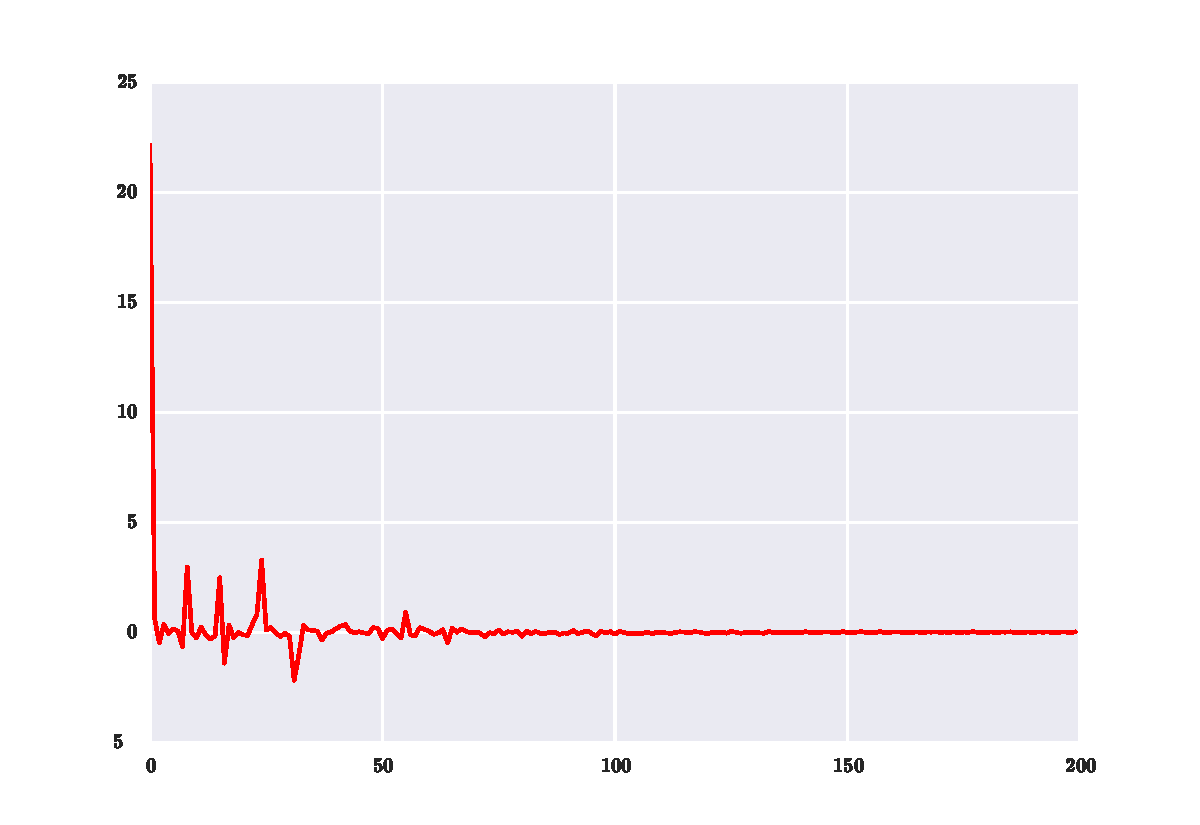
\includegraphics[width=0.25\textwidth]{../Figures/Behaviors/33.pdf}
\end{center}
\end{block}
\end{minipage}

\begin{minipage}{\textwidth}
\begin{block}{Voxels touching ground per timestep}
\begin{center}
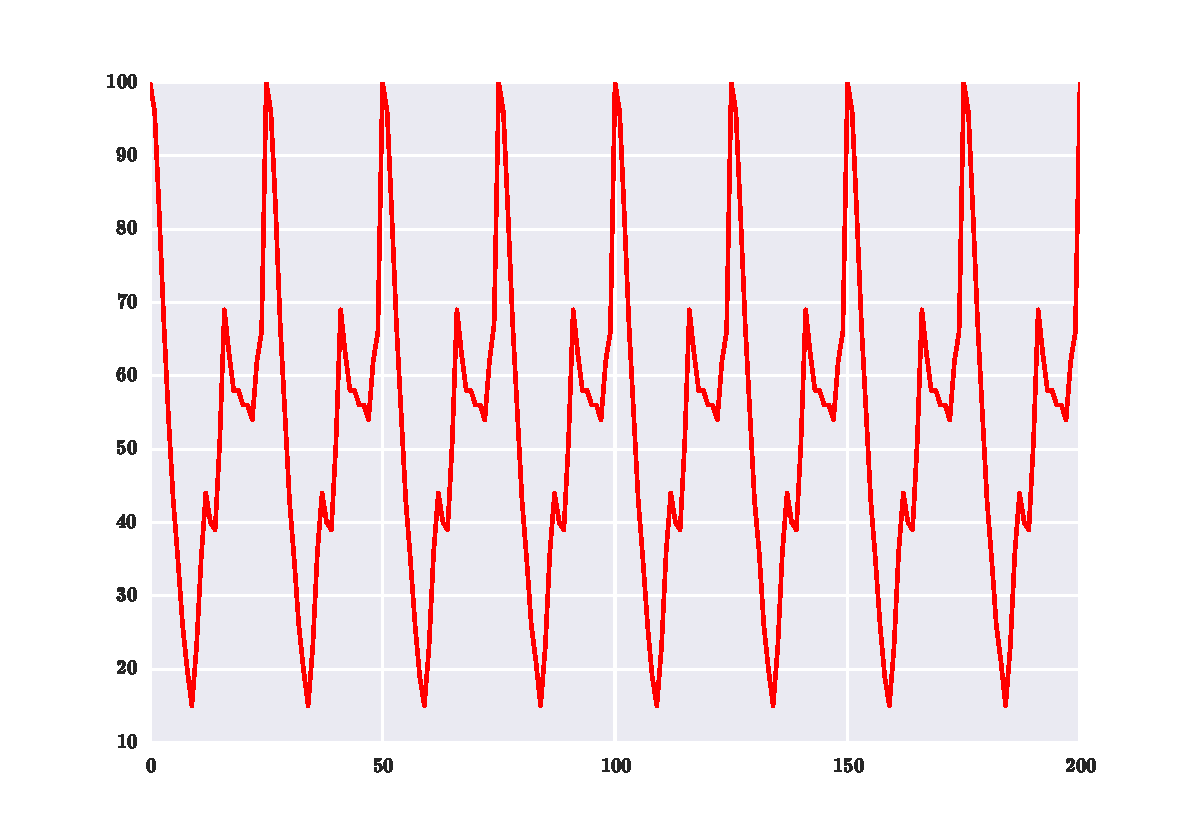
\includegraphics[width=0.25\textwidth]{../Figures/Behaviors/40.pdf}
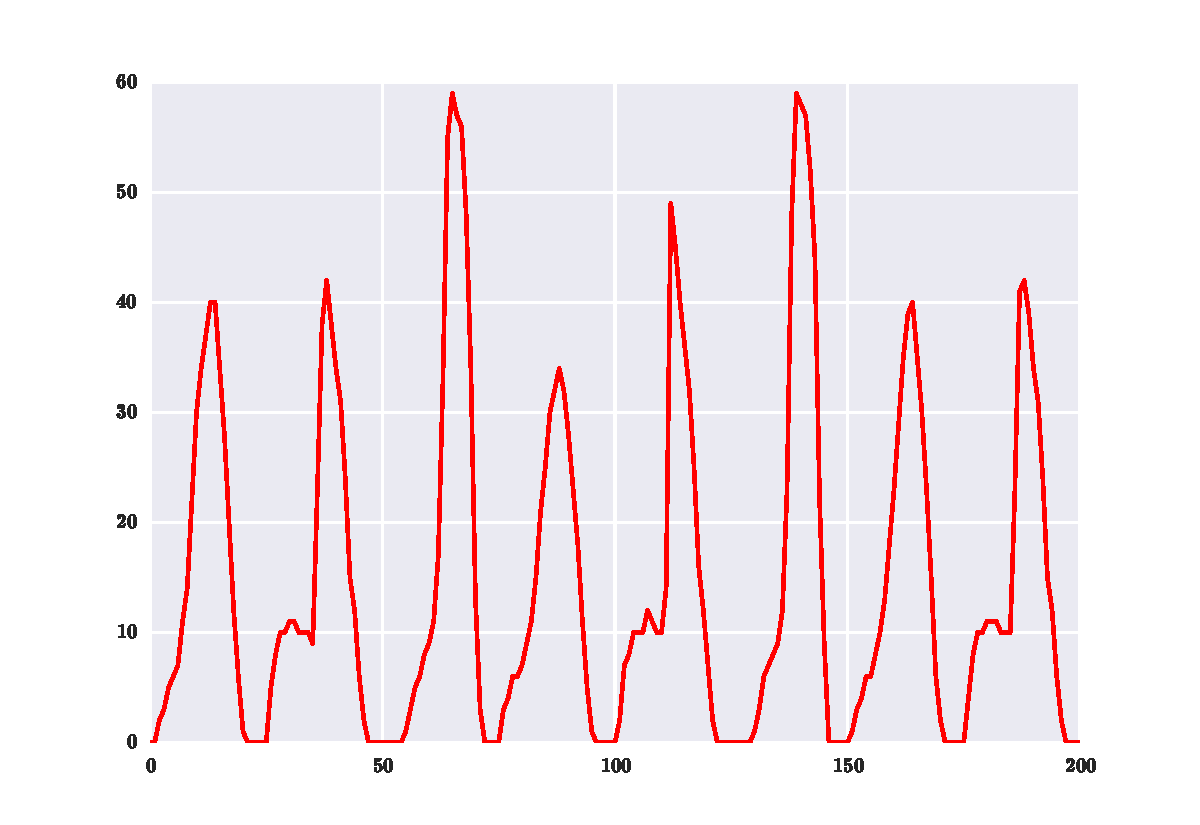
\includegraphics[width=0.25\textwidth]{../Figures/Behaviors/41.pdf}
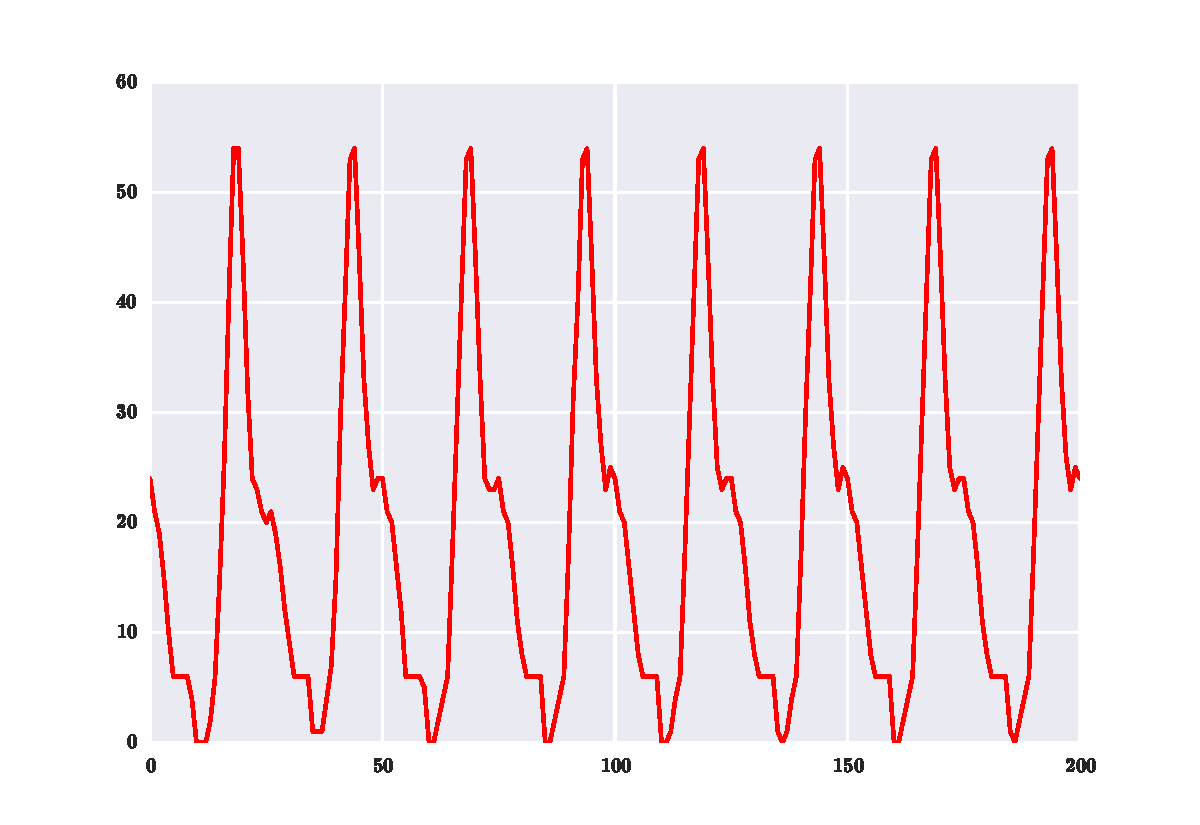
\includegraphics[width=0.25\textwidth]{../Figures/Behaviors/42.pdf}
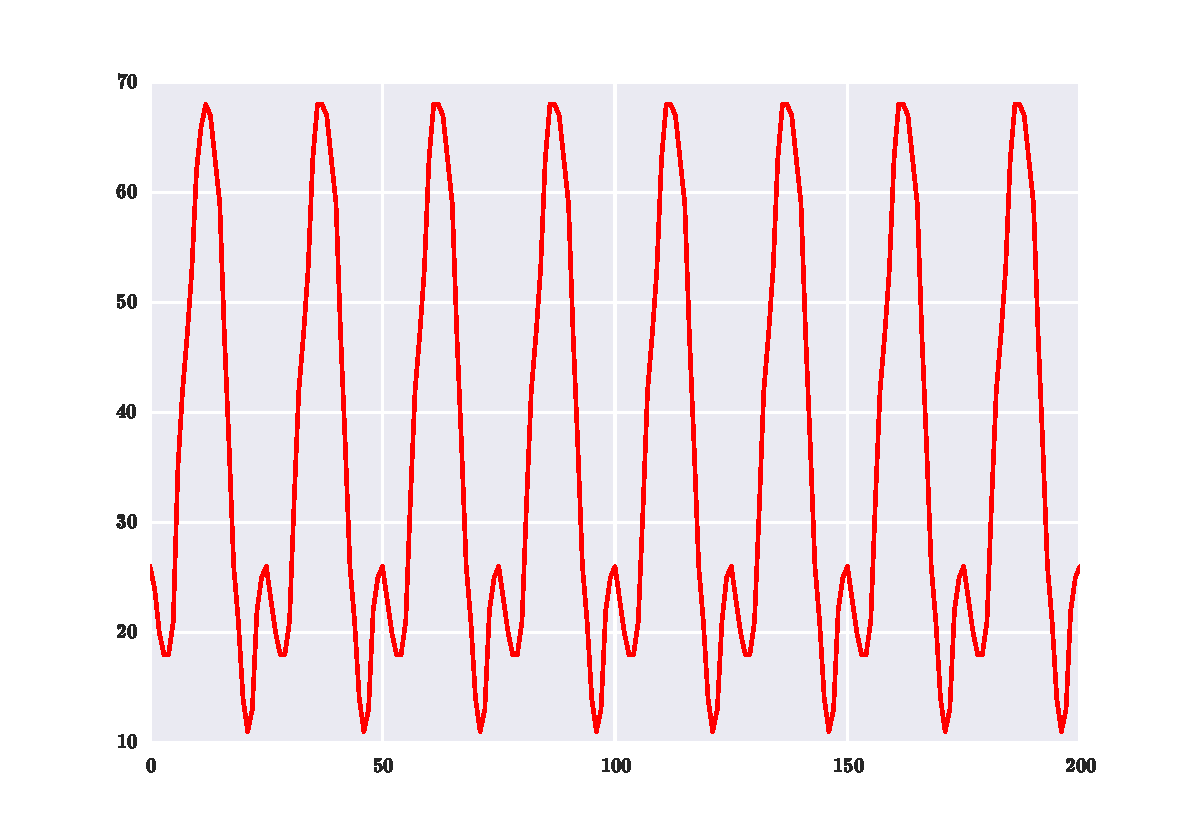
\includegraphics[width=0.25\textwidth]{../Figures/Behaviors/43.pdf}
\end{center}
\end{block}
\begin{block}{Kinetic energy per timestep}
\begin{center}
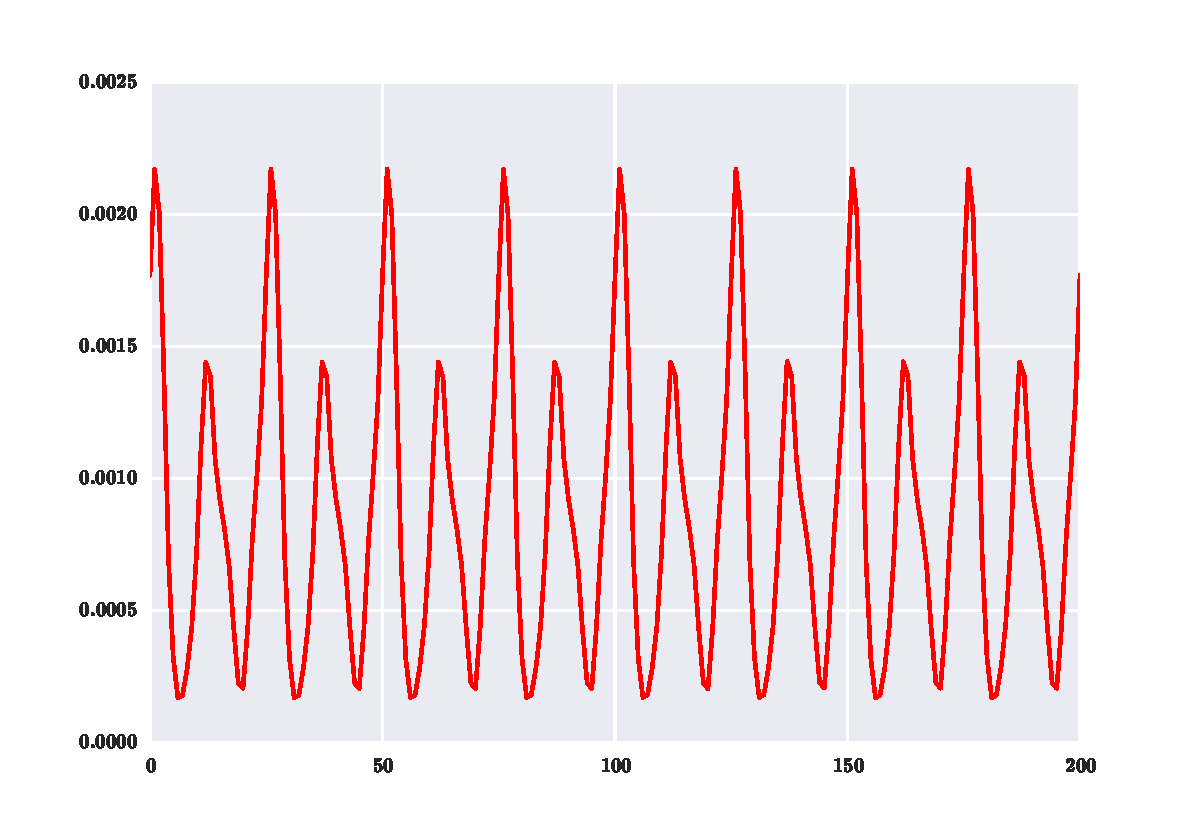
\includegraphics[width=0.25\textwidth]{../Figures/Behaviors/50.pdf}
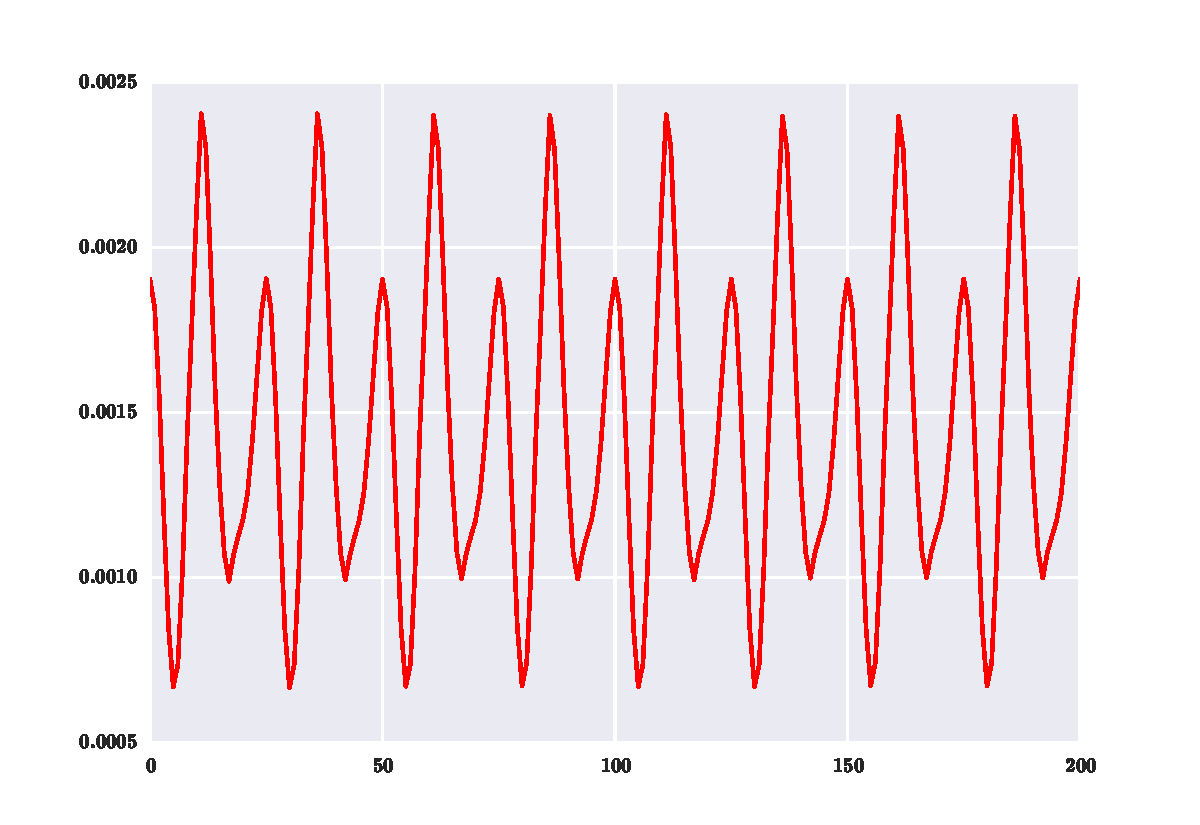
\includegraphics[width=0.25\textwidth]{../Figures/Behaviors/51.pdf}
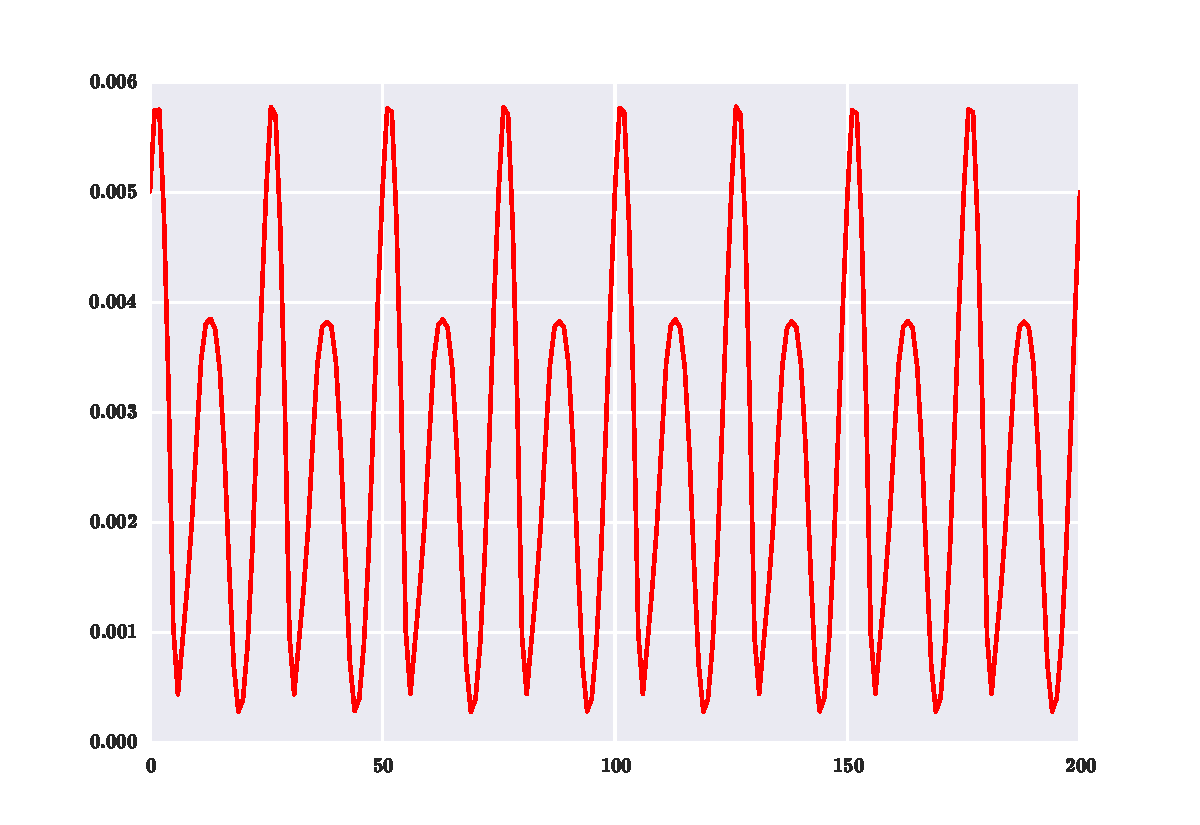
\includegraphics[width=0.25\textwidth]{../Figures/Behaviors/52.pdf}
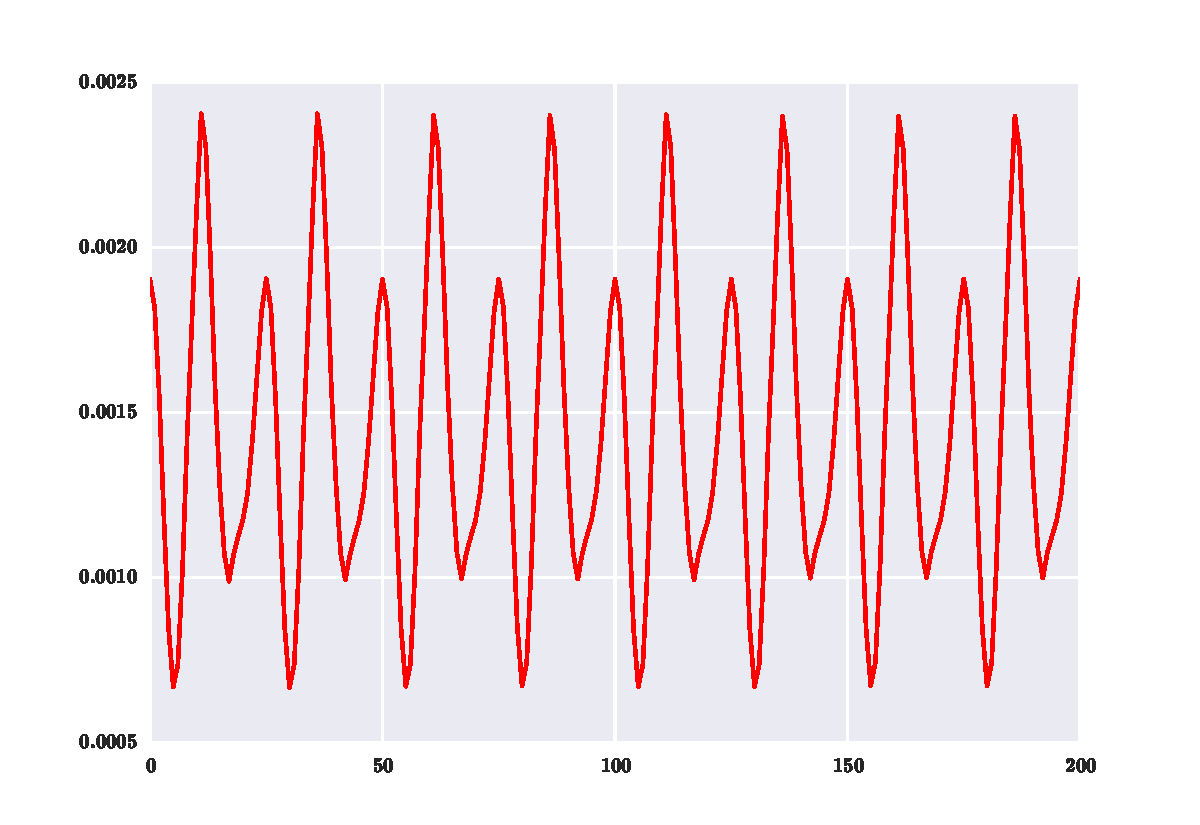
\includegraphics[width=0.25\textwidth]{../Figures/Behaviors/53.pdf}
\end{center}
\end{block}
\end{minipage}

\begin{minipage}{\textwidth}
\begin{block}{Maximum pressure per timestep}
\begin{center}
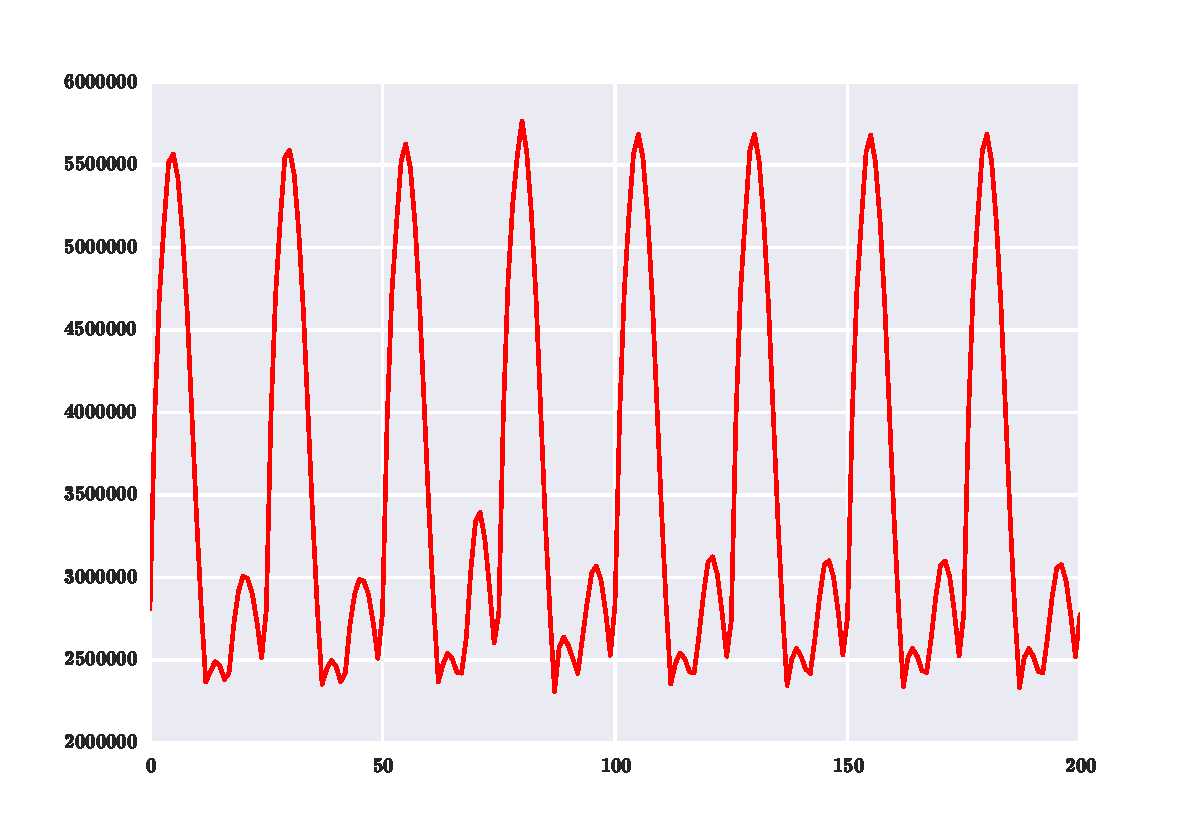
\includegraphics[width=0.25\textwidth]{../Figures/Behaviors/60.pdf}
\includegraphics[width=0.25\textwidth]{../Figures/Behaviors/61.pdf}
\includegraphics[width=0.25\textwidth]{../Figures/Behaviors/62.pdf}
\includegraphics[width=0.25\textwidth]{../Figures/Behaviors/63.pdf}
\end{center}
\end{block}
\end{minipage}

\end{frame}



\section{Results}

\begin{frame}[allowframebreaks]{Results}

\begin{minipage}{\textwidth}
\begin{block}{Fitness, Novelty, Random, Direct GA}
\includegraphics[width=1.0\textwidth]{../Figures/Results/FitNovRandomDirectSize5.pdf}
\end{block}
\end{minipage}

\begin{minipage}{\textwidth}
\begin{block}{Fitness, Novelty, Direct GA}
\includegraphics[width=1.0\textwidth]{../Figures/Results/FitvsNovVsDirSize10.pdf}
\end{block}
\end{minipage}

\begin{minipage}{\textwidth}
\vspace{0.5cm}
\begin{block}{$10$ individual runs for fitness-novelty based search.}
\includegraphics[width=0.5\textwidth]{../Figures/Results/indRunsSize10Fitness.pdf}	
\includegraphics[width=0.5\textwidth]{../Figures/Results/indRunsSize10Novelty.pdf}
\end{block}
\end{minipage}

\newpage
\begin{minipage}{\textwidth}
\begin{block}{Novelty Search - Champions every 100 generations:}
\includegraphics[width=0.2\textwidth]{../Figures/Robots/n_3_g_100.jpg}
\includegraphics[width=0.2\textwidth]{../Figures/Robots/n_3_g_200.jpg}
\includegraphics[width=0.2\textwidth]{../Figures/Robots/n_3_g_300.jpg}
\includegraphics[width=0.2\textwidth]{../Figures/Robots/n_3_g_400.jpg}
\includegraphics[width=0.2\textwidth]{../Figures/Robots/n_3_g_500.jpg}\\
\includegraphics[width=0.2\textwidth]{../Figures/Robots/n_3_g_600.jpg}
\includegraphics[width=0.2\textwidth]{../Figures/Robots/n_3_g_700.jpg}
\includegraphics[width=0.2\textwidth]{../Figures/Robots/n_3_g_800.jpg}
\includegraphics[width=0.2\textwidth]{../Figures/Robots/n_3_g_900.jpg}
\includegraphics[width=0.2\textwidth]{../Figures/Robots/n_3_g_1000.jpg}
\end{block}

\begin{block}{Fitness-based Search - Champions every 100 generations:}
\includegraphics[width=0.2\textwidth]{../Figures/Robots/f_3_g_100.jpg}
\includegraphics[width=0.2\textwidth]{../Figures/Robots/f_3_g_200.jpg}
\includegraphics[width=0.2\textwidth]{../Figures/Robots/f_3_g_300.jpg}
\includegraphics[width=0.2\textwidth]{../Figures/Robots/f_3_g_400.jpg}
\includegraphics[width=0.2\textwidth]{../Figures/Robots/f_3_g_500.jpg}\\
\includegraphics[width=0.2\textwidth]{../Figures/Robots/f_3_g_600.jpg}
\includegraphics[width=0.2\textwidth]{../Figures/Robots/f_3_g_700.jpg}
\includegraphics[width=0.2\textwidth]{../Figures/Robots/f_3_g_800.jpg}
\includegraphics[width=0.2\textwidth]{../Figures/Robots/f_3_g_900.jpg}
\includegraphics[width=0.2\textwidth]{../Figures/Robots/f_3_g_1000.jpg}
\end{block}
\end{minipage}

\begin{minipage}{\textwidth}
\begin{block}{Novelty Search - Champions every 100 generations:}
\includegraphics[width=0.2\textwidth]{../Figures/Robots/n_4_g_100.jpg}
\includegraphics[width=0.2\textwidth]{../Figures/Robots/n_4_g_200.jpg}
\includegraphics[width=0.2\textwidth]{../Figures/Robots/n_4_g_300.jpg}
\includegraphics[width=0.2\textwidth]{../Figures/Robots/n_4_g_400.jpg}
\includegraphics[width=0.2\textwidth]{../Figures/Robots/n_4_g_500.jpg}\\
\includegraphics[width=0.2\textwidth]{../Figures/Robots/n_4_g_600.jpg}
\includegraphics[width=0.2\textwidth]{../Figures/Robots/n_4_g_700.jpg}
\includegraphics[width=0.2\textwidth]{../Figures/Robots/n_4_g_800.jpg}
\includegraphics[width=0.2\textwidth]{../Figures/Robots/n_4_g_900.jpg}
\includegraphics[width=0.2\textwidth]{../Figures/Robots/n_4_g_1000.jpg}
\end{block}

\begin{block}{Fitness-based Search - Champions every 100 generations:}
\includegraphics[width=0.2\textwidth]{../Figures/Robots/f_4_g_100.jpg}
\includegraphics[width=0.2\textwidth]{../Figures/Robots/f_4_g_200.jpg}
\includegraphics[width=0.2\textwidth]{../Figures/Robots/f_4_g_300.jpg}
\includegraphics[width=0.2\textwidth]{../Figures/Robots/f_4_g_400.jpg}
\includegraphics[width=0.2\textwidth]{../Figures/Robots/f_4_g_500.jpg}\\
\includegraphics[width=0.2\textwidth]{../Figures/Robots/f_4_g_600.jpg}
\includegraphics[width=0.2\textwidth]{../Figures/Robots/f_4_g_700.jpg}
\includegraphics[width=0.2\textwidth]{../Figures/Robots/f_4_g_800.jpg}
\includegraphics[width=0.2\textwidth]{../Figures/Robots/f_4_g_900.jpg}
\includegraphics[width=0.2\textwidth]{../Figures/Robots/f_4_g_1000.jpg}
\end{block}
\end{minipage}

\begin{minipage}{\textwidth}
\begin{block}{Fitness of the generation champion (best individual) per generation}
\includegraphics[width=1.0\textwidth]{../Figures/Results/AvgGenerChampNoveltyFitnessSize5.pdf}
\end{block}
\end{minipage}

\begin{minipage}{\textwidth}
\begin{block}{Novelty Vs. Fitness, distributions of average population's fitness per generation}
\includegraphics[width=1.0\textwidth]{../Figures/Results/ViolinPlotsAvgGenFitSize5.pdf}
\end{block}
\end{minipage}

\begin{minipage}{\textwidth}
\begin{block}{Novelty Vs. Fitness, number of novel behaviors}
\includegraphics[width=1.0\textwidth]{../Figures/Results/novelIndividualsFitNovComp.pdf}
\end{block}
\end{minipage}

\begin{minipage}{\textwidth}
\begin{block}{Penalizing actuated materials, \textit{Behavior}: 2D trajectories}
\includegraphics[width=1.0\textwidth]{../Figures/Results/FitNovSize5Pen2.pdf}
\end{block}
\end{minipage}

\begin{minipage}{\textwidth}
\begin{block}{Novelty search - The novelty is computed as the average distance from the $K$-nearest behaviors.}
\includegraphics[width=1.0\textwidth]{../Figures/Results/KnnExperimentSize5.pdf}
\end{block}
\end{minipage}

\begin{minipage}{\textwidth}
\begin{block}{Local competition (global fitness, global novelty, local novelty)}
\includegraphics[width=1.0\textwidth]{../Figures/Results/NoveltyCompetitionsSize5.pdf}
\end{block}
\end{minipage}

\begin{minipage}{\textwidth}
\begin{block}{Local competition is held among the complete population of each species.}
\includegraphics[width=1.0\textwidth]{../Figures/Results/fitComp100percent.pdf}
\end{block}
\end{minipage}

%\begin{minipage}{\textwidth}
%\begin{block}{}
%\includegraphics[width=1.0\textwidth]{../Figures/Results/CopyFitChampions5.pdf}
%\end{block}
%\end{minipage}

\begin{minipage}{\textwidth}
\begin{block}{}
\includegraphics[width=1.0\textwidth]{../Figures/Results/CopyFitChampions10.pdf}
\end{block}
\end{minipage}
\end{frame}

\section{References}

\begin{frame}[allowframebreaks]{References}
\bibliographystyle{plain}
\bibliography{ref}
\end{frame}

\end{document}
